\subsection{\texorpdfstring{The spaces \(E_{A}\) (A bounded)}{The spaces E\_\{A\} (A bounded)}}

Let E be a locally convex space and A be a convex balanced subset of E. We recall that \(E_{A}\) denotes the vector space generated by A, with \(p_{A}\) the gauge of A, as the semi-norm (II, p.~26, Example 3). We verify immediately that the canonical injection of \(E_{A}\) into E is continuous if and only if A is bounded. If, in addition, E is Hausdorff, a bounded set A does not contain a line (III, p.~2, Remark 4) and so \(p_{A}\) is a norm (II, loc. cit.).

We shall say that a uniform space X is semi-complete if every Cauchy sequence in X is convergent. A complete uniform space is semi-complete; but the converse is not always true (GT, II, § 4, exerc. 4); however, a metrizable semi-complete space is complete (GT, IX, § 2, No.~6, prop. 9).

PROPOSITION 8. --- Let E be a Hausdorff locally convex space and let A be a closed, balanced, bounded and convex subset of E. Let \((x_{n})\) be a Cauchy sequence in \(E_{A}\) . Then this sequence converges in \(E_{A}\) if and only if it converges in E.

The canonical injection from \(E_{A}\) into E is continuous. Hence, if \((x_{n})\) converges in \(E_{A}\) , it converges in E. Conversely, suppose \((x_{n})\) converges to y in E. There exists an increasing sequence of integers \((n_{k})\) such that \(p_{\mathbf{A}}(x_{m}-x_{n}) \leqslant 2^{-k-1}\) if \(m \geqslant n_{k}\) and \(n \geqslant n_{k}\) . Therefore the sequence \((x_{n_{k}} + 2^{-k}\mathbf{A})\) is decreasing. Since A is closed in E, we have \(y \in \bigcap_{k} (x_{n_{k}} + 2^{-k}\mathbf{A})\) , which proves that \((x_{n_{k}})\) , hence \((x_{n})\) , converges to y in \(E_{A}\) .

COROLLARY. --- If A is semi-complete (in particular, complete) then \(E_{A}\) is a Banach space.

In fact, a Cauchy sequence in \(E_{A}\) is also a Cauchy sequence for the topology of E and is contained in a set homothetic to A, hence converges in E.

\subsection{Complete bounded sets and quasi-complete spaces}

DEFINITION 6. --- A locally convex space E is said to be quasi-complete if every closed and bounded subset of E is complete (for the uniform structure induced by that of E).

A complete locally convex space is quasi-complete, but the converse is not always true. * For example, if E is an infinite dimensional Hilbert space, or more generally, an infinite dimensional reflexive Banach space, then E with its weakened topology is quasi-complete but not complete (II, p.~51, prop. 9). *

A quasi-complete space is semi-complete, since every Cauchy sequence is contained in a closed and bounded subset (III, p.~3, corollary and prop. 1). In particular, a locally convex metrizable and quasi-complete space is complete.

In a Hausdorff quasi-complete space, the closure and the closed convex balanced envelope of a precompact subset are compact; in fact, they are precompact (II, p.~25, prop. 3), and complete being closed and bounded (III, p.~3, prop. 2).

PROPOSITION 9. --- (i) A closed vector subspace of a quasi-complete locally convex space is quasi-complete.

\begin{enumerate}
\def\labelenumi{(\roman{enumi})}
\setcounter{enumi}{1}
\item
  The product of quasi-complete locally convex spaces is quasi-complete.
\item
  The topological direct sum of quasi-complete locally convex spaces is quasi-complete.
\item
  A locally convex space which is the strict inductive limit of a sequence of closed quasi-complete subspaces is quasi-complete.
\end{enumerate}

Assertion (i) follows from Remark 2 (III, p.~2), (ii) from III, p.~4, cor. 2, (iii) from prop. 5 (III, p.~5) and (iv) from prop. 6 (III, p.~5).

We shall see later that the quotient space of a quasi-complete locally convex space by a closed vector space is not necessarily quasi-complete (IV, p.~63, exerc. 10).

PROPOSITION 10. --- Let E be a locally convex space, M a vector subspace of E such that every point of E is in the closure of a bounded subset of M. Then every continuous linear mapping f from M into a Hausdorff quasi-complete locally convex space F uniquely extends to a continuous linear mapping from E into F.

The hypothesis implies that M is dense in E, hence f extends uniquely to a continuous linear mapping f from E into the completion \(\hat{F}\) of F (GT, III, § 3, No.~4, corollary). But every \(x \in F\) lies in the closure of a bounded subset B of M; hence \(\hat{f}(x)\) is in the closure of \(f(\mathbf{B})\) in \(\hat{F}\) . But \(f(\mathbf{B})\) is bounded in F, hence its closure in F is complete, and coincides with its closure in \(\hat{F}\) . This proves that \(\hat{f}(x) \in \mathbf{F}\) .

\subsection{Examples}

\begin{enumerate}
\def\labelenumi{\alph{enumi})}
\tightlist
\item
  Let X be a topological space. Let \(\mathcal{R}(\mathrm{X})\) , the vector space of numerical (finite) functions on X be assigned the topology of compact convergence (GT, X, §1, No.~3): this is the coarsest topology for which the restriction mappings \(\mathcal{R}(\mathrm{X}) \to \mathcal{R}(\mathrm{H})\) are continuous (where H runs through the family of compact subsets of X and where \(\mathcal{R}(\mathrm{H})\) is assigned the topology of uniform convergence). Cor. 3 of III, p.~4 shows that a subset A of \(\mathcal{R}(\mathrm{X})\) is bounded if and only if, for every compact subset H of X, the set of restrictions to H of functions belonging to A is uniformly bounded.
\end{enumerate}

* b) (Spaces of infinitely differentiable functions.) Let \(n \geqslant 1\) be an integer. For every open set U in \(\mathbf{R}^n\) , let \(\mathcal{C}^\infty(\mathrm{U})\) denote the vector space of infinitely differentiable functions on U (VAR, R, 2.3). Let \(f\) be in \(\mathcal{C}^\infty(\mathrm{U})\) . For every multi-index \(\alpha = (\alpha_1, \dots, \alpha_n)\) in \(\mathbf{N}^n\) , \(\partial^\alpha f\) denotes the partial derivative \(\partial^{|\alpha|} f / \partial x_1^{\alpha_1} \dots \partial x_n^{\alpha_1}\) ; this is a continuous function on U (VAR, R, 2.3 and 2.4). For every integer \(m \geqslant 0\) , and every compact subset H of U, set

\[
p_{m,\mathrm{H}}(f) = \sup_{\substack{|\alpha |\leqslant m\\ x\in \mathrm{H}}}\left|\partial^{\alpha}f(x)\right|.\tag{1}
\]

Then \(p_{m,\mathrm{H}}\) is a semi-norm on \(\mathcal{C}^{\infty}(\mathrm{U})\) .

Let \(\mathcal{C}^{\infty}(\mathrm{U})\) be assigned the topology defined by the semi-norms \(p_{m,\mathrm{H}}\) . This is the coarsest of the topologies for which the mappings \(f\to \partial^{\alpha}f\) from \(\mathcal{C}^{\infty}(\mathrm{U})\) into \(\mathcal{R}(\mathrm{U})\) are continuous, where \(\mathcal{R}(\mathrm{U})\) is assigned the topology of compact convergence. There exists an increasing sequence of compact subsets \((\mathrm{H}_n)_{n\geqslant 0}\) of U whose interiors cover U; the family of semi-norms \(p_{m,\mathrm{H}_n}\) defines the topology of \(\mathcal{C}^{\infty}(\mathrm{U})\) , which then becomes a locally convex metrizable space. The space \(\mathcal{C}^{\infty}(\mathrm{U})\) is complete; in other words, it is a Fréchet space (II, p.~24): in fact, let \((f_k)\) be a Cauchy sequence in \(\mathcal{C}^{\infty}(\mathrm{U})\) ; for every \(\alpha \in \mathbf{N}^n\) , the sequence \((\partial^{\alpha}f_k)\) converges in the complete space \(\mathcal{R}(\mathrm{U})\) (TG, X, §1, No.~5, th. 1) to a continuous function \(g_{\alpha}\) . By induction on \(|\alpha|\) , we deduce from th. 1 of FVR, II, p.~2 that \(g_{\alpha} = \partial^{\alpha}g_{0}\) for every \(\alpha \in \mathbf{N}^n\) . In other words, the sequence \((f_k)\) converges to \(g_0\) in \(\mathcal{C}^{\infty}(\mathrm{U})\) .

Let A be a subset of \(\mathcal{C}^{\infty}(\mathrm{U})\) . In order that A be bounded, it is necessary and sufficient that the number \(\sup_{f\in \mathbf{A}}p_{m,\mathrm{H}}(f)\) is finite for every integer \(m\geqslant 0\) and for every

  compact subset H of U; this condition means that for every \(\alpha\in \mathbf{N}^{n}\) , the set of functions \(\partial^{\alpha}f|H\) for \(f\in A\) is uniformly bounded for every compact \(H\subset U\) .

Let \(\mathrm{H} \subset \mathrm{U}\) be compact. We denote by \(\mathcal{C}_{\mathrm{H}}^{\infty}(\mathrm{U})\) the subspace of \(\mathcal{C}^{\infty}(\mathrm{U})\) consisting of those functions whose support lies in \(\mathrm{H}\) . The space \(\mathcal{C}_{\circ}^{\infty}(\mathrm{U})\) of infinitely differentiable functions with compact support in \(\mathrm{U}\) is the directed increasing union of subspaces \(\mathcal{C}_{\mathrm{H}}^{\infty}(\mathrm{U})\) where \(\mathrm{H}\) runs through the family of compact subsets of \(\mathrm{U}\) . Each space \(\mathcal{C}_{\mathrm{H}}^{\infty}(\mathrm{U})\) will be assigned the topology induced by that of \(\mathcal{C}^{\infty}(\mathrm{U})\) , and \(\mathcal{C}_{\circ}^{\infty}(\mathrm{U})\) with the corresponding inductive limit topology. If the sets \(\mathrm{H}_n\) are such that their interiors form a cover of \(\mathrm{U}\) , then the space \(\mathcal{C}_{\circ}^{\infty}(\mathrm{U})\) is the strict inductive limit of the Fréchet spaces \(\mathcal{C}_{\mathrm{H}_n}^\infty (\mathrm{U})\) ; it is therefore complete (II, p.~32, prop. 9) and every bounded subset of \(\mathcal{C}_{\circ}^{\infty}(\mathrm{U})\) is contained in one of the subspaces \(\mathcal{C}_{\mathrm{H}_n}^\infty (\mathrm{U})\) (III, p.~5, prop. 6). *

\begin{enumerate}
\def\labelenumi{\alph{enumi})}
\setcounter{enumi}{2}
\tightlist
\item
  (Gevrey's spaces.) Let I be a compact interval in \(\mathbf{R}\) . For every integer \(n \geqslant 0\) , \(\mathrm{D}^n f\) denotes the \(n\) th derivative of a numerical function \(f\) defined on I (whenever this derivative exists). Let \(s \geqslant 1\) and \(\mathbf{M} \geqslant 0\) be two real numbers. Let \(\mathcal{G}_{s,\mathbf{M}}(\mathrm{I})\) denote the vector space of those infinitely differentiable functions \(f\) on I (FVR, I, p.~28) for which the sequence \((|\mathrm{D}^n f| / \mathrm{M}^n (n!)^s)_{n \geqslant 0}\) is bounded in the space \(\mathcal{C}(\mathrm{I})\) of all continuous functions on I (with the topology of uniform convergence). The space \(\mathcal{G}_{s,\mathbf{M}}(\mathrm{I})\) is a Banach space with the norm
\end{enumerate}

\[
\| f \| _ {s, \mathbf {M}} = \sup _ {n \geqslant 0, x \in \mathrm{I}} | \mathrm{D} ^ {n} f (x) | / \mathrm{M} ^ {n} (n!) ^ {s}.
\]

For \(\mathbf{M} \leqslant \mathbf{M}'\) , we have \(\mathcal{G}_{s,\mathbf{M}}(\mathrm{I}) \subset \mathcal{G}_{s,\mathbf{M}'}(\mathrm{I})\) , and

\[
\| f \| _ {s, \mathbf {M} ^ {\prime}} \leqslant \| f \| _ {s, \mathbf {M}}
\]

for every \(f \in \mathcal{G}_{s,\mathsf{M}}(\mathrm{I})\) . Let \(\mathcal{G}_s(\mathrm{I})\) denote the union of the spaces \(\mathcal{G}_{s,\mathsf{M}}(\mathrm{I})\) and endow it with the inductive limit topology of the topologies of \(\mathcal{G}_{s,\mathsf{M}}(\mathrm{I})\) .

Let \(M < M'\) and let B be the unit ball (closed) in \(\mathcal{G}_{s,M}(I)\) . We will prove that B is a compact subset of the Banach space \(\mathcal{G}_{s,M'}(I)\) . It is clear that B is closed in \(\mathcal{G}_{s,M'}(I)\) and so it is enough to prove that B is precompact in \(\mathcal{G}_{s,M'}(I)\) . Let \(\varepsilon > 0\) and let N be a positive integer such that \((M/M')^N \leqslant \varepsilon/2\) . Let k be a positive integer; the set of all functions \(D^{k+1}f\) , as f ranges over B, is bounded in \(\mathcal{C}(I)\) , hence the set of all functions \(D^k f\) , as f ranges over B, is relatively compact in \(\mathcal{C}(I)\) : this follows from the theorem of finite increments (FVR, I, p.~23, cor. 1) and from Ascoli's theorem (GT, X, § 2, No.~5). We define a norm on \(\mathcal{G}_{s,M}(I)\) by

\[
q(f) = \sup_{\substack{0\leqslant n\leqslant \mathbf{N}\\ x\in \mathrm{I}}}\big|\mathrm{D}^{n}f(x)\big| / \mathrm{M}^{\prime n}(n!)^{s}  .
\]

The above argument shows that B is precompact for the topology associated with the norm q; in other words, there exists a finite subset C of B such that for every \(f \in B\) , there exists \(g \in C\) such that \(q(f - g) \leqslant \varepsilon\) . Finally, for every n \textgreater{} N, we have

\[
\left| \mathrm{D} ^ {n} f (x) - \mathrm{D} ^ {n} g (x) \right| / \mathrm{M} ^ {\prime n} (n!) ^ {s} \leqslant 2 (\mathrm{M} / \mathrm{M} ^ {\prime}) ^ {n} \leqslant \varepsilon ,
\]

from which we get \(\| f - g\| \leqslant \varepsilon\) . This proves that B is precompact in \(\mathcal{G}_{s,M'}(I)\) .

The space \(\mathcal{G}_s(\mathrm{I})\) is the inductive limit of the spaces \(\mathcal{G}_{s,k}(\mathrm{I})\) as \(k\) ranges over \(\mathbf{N}\) ; by prop. 7 (III, p.~6) every bounded subset of \(\mathcal{G}_s(\mathrm{I})\) is contained in one of the spaces \(\mathcal{G}_{s,k}(\mathrm{I})\) and is relatively compact in this space.

* \(d\) ) (Spaces of holomorphic functions.) Let \(n \geqslant 1\) be an integer. For every open subset U of \(\mathbf{C}^n\) , \(\mathcal{H}(\mathrm{U})\) denotes the space of functions holomorphic in U, and is assigned the topology of compact convergence in U. For every compact subset L of \(\mathbf{C}^n\) , \(\mathcal{H}(\mathrm{L})\) denotes the space of germs of holomorphic functions in a neighbourhood of L; we endow this space with the finest locally convex topology for which the canonical mappings \(\pi_{\mathrm{U}}:\mathcal{H}(\mathrm{U})\to\mathcal{H}(\mathrm{L})\) are continuous, where U ranges over the set of open neighbourhoods of L.

For every integer \(m \geqslant 1\) , let \(U_{m}\) be the set of points of \(C^{n}\) which are at a distance \textless{} 1/m from L. It can be shown that the canonical mapping \(\pi_{U_{m}}\) from \(\mathcal{H}(U_{m})\) into \(\mathcal{H}(L)\) is injective, and that the restriction mapping from \(\mathcal{H}(U_{m})\) into \(\mathcal{H}(U_{p})\) is compact for \(p \geqslant m\) . We can then apply prop. 7 (III, p.~6). Let A be a bounded subset of \(\mathcal{H}(L)\) ; then there exists an integer \(m \geqslant 1\) such that A consists of germs of functions in a neighbourhood of L, belonging to a bounded set B in \(\mathcal{H}(U_{m})\) . Moreover, a mapping \(\phi\) from \(\mathcal{H}(L)\) into a topological space T is continuous if and only if the mapping \(\phi \circ \pi_{U}\) from \(\mathcal{H}(U)\) into T is continuous for every open neighbourhood U of L. *

\section{BORNOLOGICAL SPACES}

In this paragraph, E denotes a locally convex space, and B its canonical bornology (III, p.~3, def. 5).

Lemma 1. --- Let G be a semi-normed space, p its semi-norm, and u a linear mapping from G into E. The following conditions are equivalent :

\begin{enumerate}
\def\labelenumi{(\roman{enumi})}
\item
  \(u\) is continuous;
\item
  the image of the unit ball of \(G\) under \(u\) is bounded in \(\mathbf{E}\) ;
\item
  for every sequence \((x_{n})\) of points of \(\mathbf{G}\) tending to 0, the sequence \((u(x_{n}))\) is bounded in E.
\end{enumerate}

It is immediate that (i) implies (ii) (III, p.~4, cor. 1) and that (ii) implies (iii). Let V be a neighbourhood of 0 in E; if \(u^{-1}(\mathrm{V})\) is not a neighbourhood of 0 in G, then there exists a sequence \((y_n)\) of points of \(\mathrm{G} - u^{-1}(\mathrm{V})\) such that \(p(y_n) \leqslant \frac{1}{n^2}\) . Hence the sequence \(x_n = ny_n\) tends to 0 in G and \(u(x_n) \notin n\mathrm{V}\) , which implies that the sequence \((u(x_n))\) is not bounded. Therefore (iii) implies (i).

PROPOSITION 1. -- The following conditions are equivalent :

\begin{enumerate}
\def\labelenumi{(\roman{enumi})}
\tightlist
\item
  Every semi-norm on \(\mathbf{E}\) which is bounded on bounded subsets of \(\mathbf{E}\) is continuous.
\end{enumerate}

(i') Every convex balanced subset of E which absorbs the bounded subsets of E (I, p.~7, def. 4) is a neighbourhood of 0 in E.

\begin{enumerate}
\def\labelenumi{(\roman{enumi})}
\setcounter{enumi}{1}
\tightlist
\item
  E is the inductive limit of the semi-normed spaces \(E_{A}\) , where A ranges over the directed increasing set of closed, convex, balanced and bounded subsets of E.
\end{enumerate}

(ii') There exists a family \((\mathrm{E}_{i})_{i\in\mathrm{I}}\) of semi-normed spaces, and for every \(i\in I\) , a linear mapping \(u_{i}:E_{i}\to E\) such that the topology of E is the finest locally convex topology for which the \(u_{i}\) are continuous.

\begin{enumerate}
\def\labelenumi{(\roman{enumi})}
\setcounter{enumi}{2}
\tightlist
\item
  For an arbitrary locally convex space F, a linear mapping \(u: E \to F\) is continuous if and only if for every sequence \((x_{n})\) of points in E tending to 0, the sequence \((u(x_{n}))\) is bounded in F.
\end{enumerate}

(iii') For an arbitrary semi-normed space \(\mathbf{F}\) , a linear mapping \(u: \mathbf{E} \to \mathbf{F}\) is continuous if and only if \(u(\mathbf{X})\) is bounded in \(\mathbf{F}\) for every bounded set \(\mathbf{X}\) in \(\mathbf{E}\) .

It is immediate that (i) and (i') are equivalent in view of the correspondence between semi-norms and convex, balanced, absorbent subsets (II, p.~20). If \(p\) is a semi-norm on E, which is continuous on each \(\mathrm{E}_{\mathrm{A}}\) , then \(p\) is bounded on bounded subsets of E; hence (i) implies (ii) (II, p.~27, prop. 5). It is clear that (ii) implies (ii').

Now let \((\mathrm{E}_{i}, u_{i})_{i\in I}\) be as in (ii') and let u be a linear mapping from E into a locally convex space F, such that \((u(x_{n}))\) is bounded in F for every sequence \((x_{n})\) of points of E tending to 0. It follows from lemma 1 of III, p.~11 that the linear mapping \(u\circ u_{i}:E_{i}\to F\) is continuous for all \(i\in I\) . Hence, if the topology of E is the finest locally convex topology for which the \(u_{i}\) are continuous, then u is continuous (II, p.~27, prop. 5). This proves that (ii') implies (iii).

It is immediate that (iii) implies (iii') (III, p.~3, cor.) Finally, if \(p\) is a semi-norm on E, which is bounded on bounded subsets of E, the condition (iii') asserts that the identity map is continuous from E into the semi-normed space (E, \(p\) ); in other words, \(p\) is continuous. This proves that (iii') implies (i).

DEFINITION 1. --- A locally convex space is said to be bornological if it satisfies the equivalent conditions of prop. 1.

Examples. --- 1) Every semi-normed space is bornological.

\begin{enumerate}
\def\labelenumi{\arabic{enumi})}
\setcounter{enumi}{1}
\item
  In particular, every finite dimensional locally convex space is bornological.
\item
  On account of the transitivity of final locally convex topologies (II, p.~28, cor. 2), we deduce at once from condition (ii') that if \((\mathrm{E}_i)_{i\in I}\) is a family of locally convex bornological spaces and if E is assigned the finest locally convex topology for which the linear mappings \(u_{i}:\mathrm{E}_{i}\to \mathrm{E}\) (for \(i\in \mathrm{I}\) ) are continuous, then E is bornological. In particular, an inductive limit, a direct sum, a quotient space of bornological spaces are bornological spaces.
\end{enumerate}

On the other hand, a closed subspace of a bornological space is not necessarily bornological (IV, p.~63, exerc. 8).

COROLLARY. --- Every Hausdorff and semi-complete bornological space is an inductive limit of Banach spaces.

In fact, the spaces \(E_{A}\) , where A is closed and bounded are Banach spaces (III, p.~8, corollary).

PROPOSITION 2. --- A locally convex metrizable space is bornological.

Suppose E is metrizable, and p a semi-norm on E which is bounded on bounded subsets of E, but which is not continuous. Let A be the set of all \(x \in E\) such that \(p(x) < 1\) . Let \((\mathrm{V}_{n})_{n \geqslant 1}\) be a decreasing sequence forming a fundamental system of neighbourhoods of 0 in E. Since p is not continuous, A is not a neighbourhood of 0; hence for every n \textgreater{} 0, we have \(A \not\subset n^{-1}V_{n}\) and there exists a point \(x_{n}\) in \(V_{n}\) , such that \(n^{-1}x_{n} \notin A\) , that is, \(p(x_{n}) \geqslant n\) . The sequence \((x_{n})\) tends to 0, hence is bounded (III, p.~3, corollary); this contradicts the hypothesis on p.

COROLLARY. --- Every Fréchet space (II, p.~24) is the inductive limit of Banach spaces.

\section{SPACES OF CONTINUOUS LINEAR MAPPINGS}

\subsection{\texorpdfstring{The spaces \(\mathcal{L}_{\mathfrak{S}}(\mathbf{E};\mathbf{F})\)}{The spaces \textbackslash mathcal\{L\}\_\{\textbackslash mathfrak\{S\}\}(\textbackslash mathbf\{E\};\textbackslash mathbf\{F\})}}

Let \(\mathbf{F}\) be a topological vector space, \(\mathbf{E}\) an arbitrary set, and \(\mathfrak{S}\) a family of subsets of \(\mathbf{E}\) . Consider the vector space \(\mathrm{F}^{\mathrm{E}}\) with the uniform structure of \(\mathfrak{S}\) -convergence (GT, X, § 1, No.~2). We know that this structure is compatible with the commutative group structure of \(\mathrm{F}^{\mathrm{E}}\) (GT, X, § 1, No.~4, cor. 2). The topology so deduced is called the \(\mathfrak{S}\) -topology. If \(\mathbf{X}\) is a subset of \(\mathrm{F}^{\mathrm{E}}\) , or more generally, a set with a mapping \(j: \mathrm{X} \to \mathrm{F}^{\mathrm{E}}\) , then the inverse image under \(j\) of the \(\mathfrak{S}\) -topology on \(\mathrm{F}^{\mathrm{E}}\) is called the \(\mathfrak{S}\) -topology on \(\mathbf{X}\) .

Remarks. --- 1) The \(\mathfrak{S}\) -topology is identical with the \(\mathfrak{S}'\) -topology, where \(\mathfrak{S}'\) denotes the bornology generated by \(\mathfrak{S}\) (III, p.~1).

\begin{enumerate}
\def\labelenumi{\arabic{enumi})}
\setcounter{enumi}{1}
\tightlist
\item
  Let \(\mathbf{M} \in \mathfrak{S}\) and let \(\mathbf{V}\) be a neighbourhood of 0 in \(\mathbf{F}\) ; let \(\mathrm{T}(\mathbf{M}, \mathbf{V})\) denote the set of all \(f \in \mathrm{F}^{\mathrm{E}}\) such that \(f(x) \in \mathbf{V}\) for every \(x \in \mathbf{M}\) . If \(\mathfrak{S}\) is stable under finite unions, the sets \(\mathrm{T}(\mathbf{M}, \mathbf{V})\) form a fundamental system of neighbourhoods of 0 for the \(\mathfrak{S}\) -topology of \(\mathrm{F}^{\mathrm{E}}\) .
\end{enumerate}

PROPOSITION 1. --- Let E be a set, S a family of subsets of E, F a topological vector space and H a vector subspace of \(F^{E}\) . In order that the S-topology be compatible with the vector space structure of H, it is necessary and sufficient that \(u(\mathbf{M})\) is bounded in F for every \(u \in H\) and every \(M \in S\) . If, moreover, F is locally convex, then the S-topology on H is locally convex.

On account of Remarks 1) and 2) above, we see that a necessary and sufficient condition for the \(\mathfrak{S}\) -topology to be compatible with the vector space structure of H is that the sets \(\mathrm{H} \cap \mathrm{T}(\mathbf{M}, \mathrm{V})\) are absorbent in H (I, p.~7, prop. 4); but this implies that for every \(u \in \mathrm{H}\) , every subset \(\mathbf{M} \in \mathfrak{S}\) , and every balanced neighbourhood V of 0 in F, there exists \(\lambda \neq 0\) such that \(u(M) \subset \lambda V\) ; that is to say (III, p.~2) that \(u(\mathbf{M})\) is bounded in F. Finally, the last assertion of the proposition follows from the fact that if V is convex, so is \(\mathrm{T}(\mathbf{M}, \mathrm{V})\) .

COROLLARY. --- Let E and F be two locally convex spaces, S a family of bounded subsets of E, and \(\mathcal{L}(E; F)\) the vector space of continuous linear mappings from E into F. Then the S-topology is compatible with the vector space structure of \(\mathcal{L}(E; F)\) and is locally convex.

It is enough to remark that if \(u\) is a continuous linear mapping from \(\mathbf{E}\) into \(\mathbf{F}\) and \(\mathbf{M}\) is a bounded subset of \(\mathbf{E}\) , then \(u(\mathbf{M})\) is bounded in \(\mathbf{F}\) (III, p.~4, cor. 1).

Given two locally convex vector spaces E and F, and a family S of bounded subsets of E, let \(\mathcal{L}_{\mathfrak{S}}(E;F)\) denote the locally convex space obtained by assigning the S-topology to \(\mathcal{L}(E;F)\) .

Examples. --- 1) If \(\mathfrak{S}\) is the set of all finite subsets of E, then the \(\mathfrak{S}\) -topology is the topology of simple convergence and the space \(\mathcal{L}_{\mathfrak{S}}(E; F)\) is also denoted by \(\mathcal{L}_s(E; F)\) . A bounded subset of \(\mathcal{L}_s(E; F)\) is called a simply bounded subset of \(\mathcal{L}(E; F)\) .

\begin{enumerate}
\def\labelenumi{\arabic{enumi})}
\setcounter{enumi}{1}
\item
  If \(\mathfrak{S}\) is the set of compact (resp. precompact, compact convex) subsets, then the \(\mathfrak{S}\) -topology is called the topology of compact (resp. precompact, compact convex) convergence and the space \(\mathcal{L}_{\mathfrak{S}}(\mathrm{E};\mathrm{F})\) is also denoted by \(\mathcal{L}_c(\mathrm{E};\mathrm{F})\) (resp. \(\mathcal{L}_{pc}(\mathrm{E};\mathrm{F}),\mathcal{L}_{cc}(\mathrm{E};\mathrm{F})\) ). (Cf. IV, p.~48, exerc. 7.)
\item
  If \(\mathfrak{S}\) is the set of all bounded subsets of E, we say that the \(\mathfrak{S}\) -topology is the topology of bounded convergence and the space \(\mathcal{L}_{\mathfrak{S}}(\mathrm{E};\mathrm{F})\) is denoted by \(\mathcal{L}_b(\mathrm{E};\mathrm{F})\) .
\item
  When \(\mathrm{F} = \mathbf{K}\) , the space \(\mathcal{L}(\mathrm{E};\mathrm{F})\) is the dual \(\mathrm{E}'\) of \(\mathrm{E}\) . We denote by \(\mathrm{E}_{\Xi}^{\prime}, \mathrm{E}_{s}^{\prime}\) etc. the space \(\mathcal{L}_{\Xi}(\mathrm{E};\mathbf{K}), \mathcal{L}_s(\mathrm{E};\mathbf{K})\) etc. The space \(\mathrm{E}_s^\prime\) (resp. \(\mathrm{E}_b^\prime\) ) is called the weak dual (resp. strong dual) of \(\mathrm{E}\) . A bounded subset of \(\mathrm{E}_s^\prime\) (resp. \(\mathrm{E}_b^\prime\) ) is said to be weakly (resp. strongly) bounded. We observe that the weak topology on \(\mathrm{E}'\) is none other than \(\sigma (\mathrm{E}',\mathrm{E})\) (II, p.~42).
\end{enumerate}

When \(\mathrm{E} = \mathrm{F}\) , we denote by \(\mathcal{L}(\mathrm{E}), \mathcal{L}_{\mathfrak{S}}(\mathrm{E})\) etc. the space \(\mathcal{L}(\mathrm{E};\mathrm{F}), \mathcal{L}_{\mathfrak{S}}(\mathrm{E};\mathrm{F})\) etc. Let \(p\) be a continuous semi-norm on \(\mathrm{F}\) and \(\mathbf{M}\) a bounded subset of \(\mathrm{E}\) . Let

\[
p _ {\mathrm{M}} (u) = \sup _ {x \in \mathrm{M}} p (u (x)).\tag{1}
\]

It is immediate that \(p_{M}\) is a semi-norm on \(\mathcal{L}(E;F)\) and that if \(\Gamma\) is a fundamental system of semi-norms on F, the family of semi-norms \(p_{M}\) , where p ranges over \(\Gamma\) and M ranges over a base for the bornology generated by S, is a fundamental system of semi-norms of \(\mathcal{L}_{\mathfrak{S}}(E;F)\) .

In particular, if E and F are semi-normed spaces, and if p (resp. q) denotes the semi-norm of E (resp. F), then the topology of bounded convergence on \(\mathcal{L}(\mathrm{E};\mathrm{F})\) is defined by the semi-norm

\[
r (u) = \sup _ {p (x) \leqslant 1} q (u (x))\tag{2}
\]

(cf.~GT, X, § 3, No.~2). When we consider \(\mathcal{L}_b(\mathrm{E};\mathrm{F})\) as a semi-normed space, we shall always, unless the contrary is expressly stated, mean the semi-norm (2). If F is a normed space, the semi-norm (2) is a norm.

Remarks. --- 3) Let A be a dense subset of the unit ball of E. In view of the continuity of u, we also have

\[
r (u) = \sup _ {x \in \mathrm{A}} q (u (x)).\tag{3}
\]

For example

\[
r (u) = \sup _ {p (x) <   1} q (u (x)).\tag{4}
\]

Since we have \(u(tx) = tu(x)\) for \(t \in \mathbf{R}\) , we also have,

\[
r (u) = \sup _ {p (x) = 1} q (u (x)) = \sup _ {p (x) \neq 0} \frac {q (u (x))}{p (x)}.\tag{5}
\]

whenever \(p \neq 0\) .

\begin{enumerate}
\def\labelenumi{\arabic{enumi})}
\setcounter{enumi}{3}
\tightlist
\item
  The formula (2) shows that the map \(u \mapsto r(u)\) is lower semi-continuous on \(\mathcal{L}_s(\mathrm{E};\mathrm{F})\) .
\end{enumerate}

PROPOSITION 2. --- Let E and F be two locally convex spaces and let S be a set of bounded subsets of E.

\begin{enumerate}
\def\labelenumi{\arabic{enumi})}
\item
  The \(\mathfrak{S}\) -topology on \(\mathcal{L}(\mathrm{E};\mathrm{F})\) is identical with the \(\mathfrak{S}\) -topology, where \(\mathfrak{S}\) denotes the smallest adapted, bornology (III, p.~3) on \(\mathrm{E}\) which contains \(\mathfrak{S}\) .
\item
  Suppose that \(\{0\}\) is not dense in \(\mathbf{F}\) and let \(\mathfrak{S}'\) be another set of bounded subsets of \(\mathbf{E}\) . Then the \(\mathfrak{S}'\) -topology is coarser than the \(\mathfrak{S}\) -topology if and only if \(\mathfrak{S}' \subset \tilde{\mathfrak{S}}\) .
\end{enumerate}

Let \(u \in \mathcal{L}(\mathrm{E};\mathrm{F})\) , \(\mathbf{M} \in \mathfrak{S}\) and let \(p\) be a continuous semi-norm on \(\mathrm{F}\) . Since \(p \circ u\) is a continuous semi-norm on \(\mathrm{E}\) , this is the same as saying that \(p \circ u\) is bounded above by 1 on \(\mathbf{M}\) or on the closed, convex balanced envelope \(\tilde{\mathbf{M}}\) of \(\mathbf{M}\) ; in other words, we have \(p_{\mathbf{M}} = p_{\tilde{\mathbf{M}}}\) . Moreover, it is clear that we have \(p_{\lambda \mathbf{M}} = \lambda p_{\mathbf{M}}\) for all \(\lambda > 0\) and \(p_{\mathbf{M} \cup \mathbf{M}'} = \sup(p_{\mathbf{M}}, p_{\mathbf{M}'})\) , from which the first assertion follows, since \(\tilde{\mathfrak{S}}\) has the set of homothetics of the closed convex balanced envelopes of finite unions of sets of \(\mathfrak{S}\) as a base.

We now prove the second assertion: first, if \(\mathbf{F}\) is the base field, it follows from the definition that the \(\tilde{\mathfrak{S}}\) -topology on \(\mathrm{E}' = \mathcal{L}(\mathrm{E};\mathrm{F})\) has as a fundamental system of neighbourhoods of 0, the set of polars of the sets of \(\tilde{\mathfrak{S}}\) . Let \(\mathbf{A}\) be a bounded subset of \(\mathbf{E}\) , whose polar \(\mathbf{A}^{\circ}\) is a neighbourhood of 0 for the \(\tilde{\mathfrak{S}}\) -topology; then there exists a closed convex balanced set \(\mathbf{B} \in \tilde{\mathfrak{S}}\) such that \(\mathbf{A}^{\circ} \supset \mathbf{B}^{\circ}\) , and so \(\mathbf{A} \subset \mathbf{B}^{\circ \circ}\) ; but by cor. 3 of II, p.~45, we have \(\mathbf{B}^{\circ \circ} = \mathbf{B}\) , and hence \(\mathbf{A} \subset \mathbf{B}\) and \(\mathbf{A} \in \tilde{\mathfrak{S}}\) . Therefore if \(\mathfrak{S}'\) is a set of bounded subsets of \(\mathbf{E}\) , the \(\mathfrak{S}'\) -topology is coarser than the \(\mathfrak{S}\) -topology on \(\mathrm{E}'\) if and only if \(\mathfrak{S}' \subset \tilde{\mathfrak{S}}\) . The general case follows immediately, since if \(y \in F\) is not in the closure of 0, we can verify that the mapping which makes \(f \in E'\) correspond to the mapping \(x \mapsto f(x)y\) is an isomorphism of the locally convex spaces \(\mathrm{E}'_{\mathfrak{S}}\) onto its image in \(\mathcal{L}_{\mathfrak{S}}(\mathrm{E};\mathrm{F})\) .

\subsection{\texorpdfstring{Condition for \(\mathcal{L}_{\mathfrak{S}}(\mathbf{E};\mathbf{F})\) to be Hausdorff}{Condition for \textbackslash mathcal\{L\}\_\{\textbackslash mathfrak\{S\}\}(\textbackslash mathbf\{E\};\textbackslash mathbf\{F\}) to be Hausdorff}}

PROPOSITION 3. -- Let E and F be two locally convex spaces, F being assumed Hausdorff, and let \(\mathfrak{S}\) be a family of bounded subsets of E. If the union A of the sets of \(\mathfrak{S}\) is total in E, then the space \(\mathcal{L}_{\mathfrak{S}}(\mathrm{E};\mathrm{F})\) is Hausdorff.

Let \(u_0\) be a non-zero element of \(\mathcal{L}(\mathrm{E};\mathrm{F})\) ; since \(u_0\) is continuous and \(\mathrm{A}\) is total in \(\mathrm{E}\) , there exists an \(x_0\) in \(\mathrm{A}\) such that \(u_0(x_0) \neq 0\) . Since \(\mathrm{F}\) is Hausdorff, there exists a neighbourhood \(\mathrm{V}\) of 0 in \(\mathrm{F}\) such that \(u_0(x_0) \notin \mathrm{V}\) . Let \(\mathbf{M} \in \mathfrak{S}\) be such that \(x_0 \in \mathbf{M}\) . Then the set \(\mathrm{U}\) of all \(u \in \mathcal{L}(\mathrm{E};\mathrm{F})\) such that \(u(\mathbf{M}) \subset \mathbf{V}\) is a neighbourhood of 0 in \(\mathcal{L}(\mathrm{E};\mathrm{F})\) , and we have \(u_0 \notin \mathrm{U}\) , hence \(\mathcal{L}(\mathrm{E};\mathrm{F})\) is Hausdorff.

In particular, the following topologies on \(\mathcal{L}(\mathrm{E};\mathrm{F})\) are Hausdorff whenever F is Hausdorff: simple convergence, compact convergence, precompact or compact convex, and bounded convergence.

\subsection{\texorpdfstring{Relations between \(\mathcal{L}(\mathbf{E};\mathbf{F})\) and \(\mathcal{L}(\hat{\mathbf{E}};\mathbf{F})\)}{Relations between \textbackslash mathcal\{L\}(\textbackslash mathbf\{E\};\textbackslash mathbf\{F\}) and \textbackslash mathcal\{L\}(\textbackslash hat\{\textbackslash mathbf\{E\}\};\textbackslash mathbf\{F\})}}

Let E and F the two Hausdorff locally convex spaces, and suppose F is complete; let \(\hat{E}\) be the completion of E. Since every continuous linear mapping u from E into F extends uniquely to a continuous linear mapping \(\overline{u}\) from \(\hat{E}\) into F, we can identify the spaces \(\mathcal{L}(E;F)\) and \(\mathcal{L}(\hat{E};F)\) by the mapping \(u\mapsto\overline{u}\) . In addition, let S be a family of bounded subsets of E; the S-topology on \(\mathcal{L}(E;F)\) coincides with the S-topology on \(\mathcal{L}(\hat{E};F)\) and also with the \(\hat{S}\) -topology, where \(\hat{S}\) denotes the family of closures in \(\hat{E}\) of sets of S.

For example, if E is normed, the topology of bounded convergence on \(\mathcal{L}(\mathrm{E};\mathrm{F})\) is identical with the topology of bounded convergence on \(\mathcal{L}(\hat{\mathrm{E}};\mathrm{F})\) : for, every bounded subset of \(\hat{E}\) is contained in the closure of a bounded subset of E. Since the unit ball of \(\hat{E}\) is the closure of the unit ball of E, it follows from formula (3) (III, p.~14) that if F is a Banach space, the map \(u\mapsto\overline{u}\) is an isometry from \(\mathcal{L}(\mathrm{E};\mathrm{F})\) onto \(\mathcal{L}(\hat{\mathrm{E}};\mathrm{F})\) .

We observe that if E is not a normed space, then there may exist bounded subsets of \(\hat{E}\) which are not contained in the closure of any bounded subset of E (for example, if E is the weak dual of an infinite dimensional Banach space); however, this is so if E is metrizable and satisfies the first axiom of countability (III, p.~39, exerc. 16).

\subsection{\texorpdfstring{Equicontinuous subsets of \(\mathcal{L}(\mathbf{E};\mathbf{F})\)}{Equicontinuous subsets of \textbackslash mathcal\{L\}(\textbackslash mathbf\{E\};\textbackslash mathbf\{F\})}}

Let \(\mathrm{E}\) and \(\mathrm{F}\) be two locally convex spaces. For a subset \(\mathrm{H}\) of \(\mathcal{L}(\mathrm{E};\mathrm{F})\) to be equicontinuous it is necessary and sufficient that it is equicontinuous at the point 0 in \(\mathrm{E}\) (I, p.~9, prop. 6); this implies that for every neighbourhood \(\mathrm{V}\) of 0 in \(\mathrm{F}\) , the set \(\bigcap_{u\in \mathrm{H}}u^{-1}(\mathrm{V})\) is a neighbourhood of 0 in \(\mathrm{E}\) ; or that for every continuous semi-norm

\(p\) on \(\mathrm{F}\) , the function \(\sup_{u\in \mathrm{H}}(p\circ u)\) is a continuous semi-norm on E. Moreover (I, p.~5),

  H is uniformly equicontinuous. We note that the convex balanced envelope of an equicontinuous subset is equicontinuous, since if p is a continuous semi-norm on F and \(\tilde{H}\) the convex balanced envelope of H, we have, for the \(u_{i}\) in H, the inequality \(p \circ (\sum_{i} \lambda_{i} u_{i}) \leqslant \sum_{i} |\lambda_{i}| \cdot (p \circ u_{i})\) , hence \(\sup_{u \in \tilde{H}} (p \circ u) = \sup_{u \in H} (p \circ u)\) .

Consequently, the family of equicontinuous subsets is a convex bornology on \(\mathcal{L}(\mathrm{E};\mathrm{F})\) (III, p.~2, def. 2).

PROPOSITION 4. --- Let E, F be two locally convex spaces, and F be Hausdorff. Let the space \(F^{E}\) of all mappings from E into F be assigned the topology of simple convergence. Then

\begin{enumerate}
\def\labelenumi{(\roman{enumi})}
\item
  The set of linear mappings from \(\mathbf{E}\) into \(\mathbf{F}\) is closed in \(\mathbf{F}^{\mathrm{E}}\) .
\item
  If \(\mathbf{H}\) is an equicontinuous subset of \(\mathcal{L}(\mathrm{E};\mathrm{F})\) , the closure \(\overline{\mathbf{H}}\) of \(\mathbf{H}\) in \(\mathrm{F}^{\mathrm{E}}\) is contained in \(\mathcal{L}(\mathrm{E};\mathrm{F})\) and is equicontinuous.
\end{enumerate}

We know that \(\overline{\mathbf{H}}\) is equicontinuous (GT, X, § 2, No.~3, prop. 6). It remains to prove the assertion (i). Let \(x, y\) be in E and \(\lambda, \mu\) in K, and let \(\mathbf{A}(x, y, \lambda, \mu)\) be the set of all \(u \in \mathbf{F}^{\mathrm{E}}\) such that

\[
u (\lambda x + \mu y) - \lambda u (x) - \mu u (y) = 0.
\]

This set is closed in \(F^{E}\) since the mapping \(u \mapsto u(x)\) from \(F^{E}\) into F is continuous for every \(x \in E\) and since \(F\) is Hausdorff. But the set of linear mappings from \(E\) into \(F\) is equal to

\[
\bigcap_ {x, y, \lambda , \mu} \mathrm{A} (x, y, \lambda , \mu).
\]

Thus this set is closed in \(F^{E}\) .

COROLLARY 1. --- For an equicontinuous subset H of \(\mathcal{L}(\mathrm{E};\mathrm{F})\) to be relatively compact in \(\mathcal{L}_s(\mathrm{E};\mathrm{F})\) , it is necessary and sufficient that for all \(x\in \mathrm{E}\) , the set \(\mathrm{H}(x)\) of all \(u(x)\) as \(u\) ranges over \(\mathrm{H}\) , is relatively compact in \(\mathrm{F}\) .

In fact, this condition is necessary and sufficient for \(\overline{\mathbf{H}}\) to be compact in \(\mathrm{F}^{\mathrm{E}}\) (GT, I, § 9, No.~5, cor.).

COROLLARY 2. --- Every equicontinuous subset of the dual E' of E is relatively compact for the weak topology \(\sigma(E', E)\) on E' (III, p.~14, Example 4).

For, if H is an equicontinuous subset of \(E'\) , \(\sup_{u\in H}|u|\) is a continuous semi-norm on E; in particular, for every \(x\in E\) , the set \(\mathrm{H}(x)\) is bounded, hence relatively compact in the field of scalars.

COROLLARY 3. --- In the strong dual \(E_{b}^{\prime}\) of a semi-normed space E, every closed ball is compact for the weak topology \(\sigma(\mathrm{E}^{\prime},\mathrm{E})\) .

This ball is also closed for \(\sigma(\mathrm{E}^{\prime},\mathrm{E})\) .

PROPOSITION 5. --- Let E and F be two locally convex spaces and let T be a total subset of E. The following uniform structures coincide on every equicontinuous subset H of \(\mathcal{L}(\mathrm{E};\mathrm{F})\) :

\begin{enumerate}
\def\labelenumi{\arabic{enumi})}
\item
  the uniform structure of simple convergence in T;
\item
  the uniform structure of simple convergence in E;
\item
  the uniform structure of convergence in the precompact subsets of E.
\end{enumerate}

We recall (III, p.~15, prop. 2) that the \(\mathfrak{S}\) -topology on \(\mathcal{L}(\mathrm{E};\mathrm{F})\) coincides with the \(\tilde{\mathfrak{S}}\) -topology, where \(\tilde{\mathfrak{S}}\) is the smallest bornology adapted to E and containing \(\mathfrak{S}\) .

In the statement of prop. 5, we can therefore replace the word « total » by « everywhere dense ». The proposition then follows from the general properties of equicontinuous sets (GT, X, § 2, No.~4, th. 1).

Examples. --- * 1) Let \(\mu\) be the Lebesgue measure on \(\mathbf{R}\) , and let E be the semi-normed space \(\mathcal{L}^p(\mu)\) ( \(1 \leqslant p < \infty\) ) (INT, IV). For every numerical function \(f\) and every real number \(h\) , let \(f_h\) be the function \(x \mapsto f(x - h)\) . Clearly the mapping \(f \mapsto f_h\) defines a linear isometry from E onto itself. If \(f\) is continuous and has compact support, then \(f_h\) converges to \(f\) uniformly, hence also in the mean of order \(p\) , as \(h\) tends to 0. Since the set \(\mathcal{K}(\mathbf{R})\) of all continuous functions with compact support is dense in E, and the set of linear isometries of E is equicontinuous, it follows from prop. 5 that for every \(f \in E\) , \(f_h\) converges in the mean of order \(p\) to \(f\) as \(h\) tends to 0.

For \(p = 1\) , consider the Fourier transform, which associates to each \(f \in \mathcal{L}^1(\mu)\) the function \(\hat{f}\) on \(\mathbf{R}\) defined by

\[
\hat {f} (y) = \int e ^ {- 2 i \pi x y} f (x) d \mu (x).
\]

The set of linear forms \(f \mapsto \hat{f}(y)\) is an equicontinuous subset of the dual of \(\mathcal{L}^1(\mu)\) . On the other hand, we know that the set \(T\) of all characteristic functions of closed bounded intervals is a total subset of \(\mathcal{L}^1(\mu)\) ; and we verify easily that for all \(f \in T\) , the Fourier transform \(\hat{f}\) is a continuous function tending to zero at infinity. We deduce that this is true for all \(f \in \mathcal{L}^1(\mu)\) (« Riemann-Lebesgue theorem »).

The relation \(\sup_{y\in \mathbb{R}}|\hat{f} (y)|\leqslant \| f\| _1\) shows that the map \(f\mapsto \hat{f}\) is a continuous map

from \(\mathcal{L}^1 (\mu)\) into the space \(\mathcal{B}(\mathbf{R})\) of all bounded functions on \(\mathbf{R}\) , with the structure of uniform convergence. Since \(\hat{f}\) is continuous for all \(f\in \mathrm{T}\) , it follows that \(\hat{f}\) is continuous for all \(f\in \mathcal{L}^1 (\mu)\) . The fact that \(\hat{f}\) tends to zero at infinity follows from the fact that the subspace \(\mathcal{C}_0(\mathbf{R})\) of all continuous functions tending to zero at infinity is closed in \(\mathcal{B}(\mathbf{R})\) .

\begin{enumerate}
\def\labelenumi{\arabic{enumi})}
\setcounter{enumi}{1}
\tightlist
\item
  Let E be the space of all continuous numerical functions on R endowed with the topology of compact convergence. Let K be a compact subset of R and let \((\mu_{n})\) be a sequence of measures on R with support in K. Suppose \(\|\mu_{n}\|\leqslant1\) for all n.~The set of the \(\mu_{n}\) is then an equicontinuous subset of \(E'\) . Therefore, if for every function \(f\in E\) , we have \(\lim_{n\to\infty}\mu_{n}(f)=0\) , the sequence of functions \(x\mapsto\int e^{itx}d\mu_{n}(t)\) converges to 0,
\end{enumerate}

uniformly on every compact subset of \(\mathbf{R}\) (since the set of functions \(t \mapsto e^{itx}\) , as \(x\) ranges over a compact subset of \(\mathbf{R}\) , is compact in E). *

COROLLARY. --- Suppose F is Hausdorff. Let H be an equicontinuous subset of \(\mathcal{L}(\mathrm{E};\mathrm{F})\) . If a filter \(\Phi\) on H converges simply to a mapping \(u_{0}\) from E into F, then \(u_{0}\) is a continuous linear mapping from E into F, and \(\Phi\) converges uniformly to \(u_{0}\) on every precompact subset of E.

The first assertion follows from prop. 4 (III, p.~16) and the second from prop. 5 (III, p.~17).

PROPOSITION 6. --- Let H be an equicontinuous subset of \(\mathcal{L}(\mathrm{E};\mathrm{F})\) . If F is metrizable and if there exists a countable total set in E, then the uniform structure on H of simple convergence in E is metrizable. If in addition, there exists a countable total set in F, then there exists a countable everywhere dense set in H (for the topology of uniform convergence on compact subsets of E).

Let \((a_{n})\) be a total sequence in E. Then the mapping \(u \mapsto (u(a_{n}))\) is an isomorphism from \(\mathcal{L}(\mathrm{E};\mathrm{F})\) , where \(\mathcal{L}(\mathrm{E};\mathrm{F})\) has the uniform structure of simple convergence on the set of the \(a_{n}\) , onto a uniform subspace of \(F^{N}\) . If F is metrizable (resp. metrizable and satisfies the first axiom of countability) then this is also true for \(F^{N}\) (GT, IX, § 2, No.~4, cor. 2 and § 2, No.~8, corollary), and the proposition follows from prop. 5 (III, p.~17).

COROLLARY 1. --- Let E be a locally convex metrizable space, and F a normed space. Suppose that E and F both satisfy the first axiom of countability. Then \(\mathcal{L}(\mathrm{E};\mathrm{F})\) is the union of a countable family of equicontinuous subsets and there exists a countable set in \(\mathcal{L}(\mathrm{E};\mathrm{F})\) which is dense for the topology of uniform convergence on precompact subsets of E.

Let B be the unit ball of F and \((\mathrm{V}_{n})\) a countable fundamental system of neighbourhoods of 0 in E. For every integer n, the set \(H_{n}\) of all \(u \in \mathcal{L}(\mathrm{E}; \mathrm{F})\) such that \(u(\mathrm{V}_{n}) \subset \mathrm{B}\) is equicontinuous and \(\mathcal{L}(\mathrm{E}; \mathrm{F})\) is the union of the \(H_{n}\) . The corollary then follows from prop. 6.

COROLLARY 2. --- Every closed ball in the dual E' of a normed space satisfying the first axiom of countability, is a compact metrizable space for the weak topology \(\sigma(\mathrm{E}',\mathrm{E})\) , and for this topology there exists a countable dense subset in E'.

This follows from prop. 6 and from III, p.~17, cor. 3.

\subsection{\texorpdfstring{Equicontinuous subsets of \(\mathbf{E}'\)}{Equicontinuous subsets of \textbackslash mathbf\{E\}\textquotesingle{}}}

In this section, E denotes a locally convex space and \(E'\) its dual. Whenever we talk of the polar \(M^{\circ}\) of a set M in E (resp. \(E'\) ), we shall always mean, unless otherwise stated, the polar of M relative to the duality between E and \(E'\) . Recall that if V is a closed convex balanced neighbourhood of 0 in E, we have \(V^{\circ\circ}=V\) (II, p.~45, cor. 3).

PROPOSITION 7. --- Let M be a subset of E'. The following conditions are equivalent :

\begin{enumerate}
\def\labelenumi{(\roman{enumi})}
\item
  M is equicontinuous;
\item
  \(\mathbf{M}\) is contained in the polar of a neighbourhood of 0 in E;
\item
  the polar of \(\mathbf{M}\) is a neighbourhood of 0 in E.
\end{enumerate}

If \(\mathbf{M}\) is equicontinuous, there exists a convex balanced neighbourhood \(V\) of 0 such that \(|u(x)| \leqslant 1\) for all \(x \in V\) and all \(u \in M\) ; then we have that \(\mathbf{M} \subset V^{\circ}\) and (i) implies (ii). With the same notations, if \(\mathbf{M} \subset V^{\circ}\) then \(\mathbf{V} \subset V^{\circ \circ} \subset M^{\circ}\) and (ii) implies (iii). Finally, if \(\mathbf{M}^{\circ}\) contains a convex balanced neighbourhood \(V\) of 0, then \(\mathbf{M} \subset M^{\circ \circ} \subset V^{\circ}\) and the relations \(x \in \varepsilon V\) , \(u \in M\) imply \(|u(x)| \leqslant \varepsilon\) for all \(\varepsilon > 0\) , which proves that (iii) implies (i).

We remark that every \(x \in E\) defines a mapping \(j(x): u \mapsto u(x)\) from \(E'\) into K. Hence we can talk of the S-topology on E, where S is a family of subsets of \(E'\) : this is the inverse image under j of the S-topology on \(K^{E'}\) . We verify immediately that if S is a convex bornology on \(E'\) , then the polars of sets of S form a fundamental system of neighbourhoods of 0 for the S-topology on E. This is so, in particular, when S is the family of equicontinuous subsets of \(E'\) and prop. 7 implies:

COROLLARY 1. --- The topology of E is identical with the topology of uniform convergence on equicontinuous subsets of E'.

More generally, let F be a locally convex space; every \(u \in \mathcal{L}(\mathrm{E}; \mathrm{F})\) defines a map \(j(u):(x, f) \mapsto f(u(x))\) from \(E \times F'\) into K (i.e.~into R or C). This enables us to define, on the space \(\mathcal{L}(\mathrm{E}; \mathrm{F})\) , the topology of uniform convergence on a set of subsets of \(E \times F'\) . In particular:

COROLLARY 2. --- Let S be a family of bounded subsets of E. The S-topology on \(\mathcal{L}(\mathrm{E};\mathrm{F})\) is the topology of uniform convergence on sets of the form \(\mathbf{A}\times\mathbf{B}\subset\mathbf{E}\times\mathbf{F}'\) , where A is in S, and B belongs to the family of equicontinuous subsets of F'.

For every \(u \in \mathcal{L}(\mathrm{E}; \mathrm{F})\) , every \(A \in S\) and every closed convex balanced neighbourhood V of 0 in F, the relation \(u(\mathrm{A}) \subset \mathrm{V}\) is equivalent to \(\ll j(u) (\mathrm{A} \times \mathrm{V}^{\circ})\) is contained in the unit ball of K \(\gg\).

PROPOSITION 8. --- Let H be a family of linear mappings from E into a locally convex space F. For H to be equicontinuous, it is necessary and sufficient that for every equicontinuous subset X in the dual F' of F, the set of linear forms \(f \circ u\) , for \(f \in X\) and \(u \in H\) , is equicontinuous.

It is obvious that the condition is necessary. Suppose it is verified, and let V be a closed convex balanced neighbourhood of 0 in F. Since \(V^{\circ}\) is equicontinuous, there exists a neighbourhood W of 0 in E such that \(\left|f(u(x))\right| \leqslant 1\) for all \(x \in W\) , \(u \in H\) and \(f \in V^{\circ}\) ; in other words, \(u(W) \subset V^{\circ\circ} = V\) for all \(u \in H\) , hence H is equicontinuous.

\subsection{The completion of a locally convex space}

THEOREM 1 (Grothendieck). --- Let E be a locally convex space, and let S be an adapted and covering bornology on E. Let \(F \subset E^{*}\) be the space of those linear forms on E whose restriction to each set belonging to S is continuous. If F is assigned the S-topology, then the canonical injection from \(E'_{S}\) into F extends to an isomorphism from the completion \(\hat{E}'_{S}\) of \(E'_{S}\) onto F.

Since every simple limit of linear forms on E is a linear form (III, p.~16, prop. 4) and since the bornology \(\mathfrak{S}\) on E is covering, it follows from GT, X, § 1, No.~6, cor. 2 that the space F with the \(\mathfrak{S}\) -topology is Hausdorff and complete. It is clear that \(E_{\mathfrak{S}}'\) is a topological vector subspace of F; hence it is enough to prove that \(E_{\mathfrak{S}}'\) is everywhere dense in F. This follows from the following lemma:

Lemma 1. --- Let A be a closed convex balanced subset of E and let u be a linear form on E whose restriction to A is continuous. Then for every \(\varepsilon > 0\) , there exists an \(x' \in E'\) such that

\[
\left| u (x) - \langle x, x ^ {\prime} \rangle \right| \leqslant \varepsilon \quad \text { for   every } \quad x \in A.
\]

Let \(\varepsilon > 0\) . There exists a closed convex balanced neighbourhood U of 0 in E such that \(|u(x)| \leqslant \varepsilon\) for all \(x \in \mathrm{U} \cap \mathrm{A}\) . We know that the polar \(\mathrm{U}^{\circ}\) of U in \(\mathrm{E}^{*}\) is contained in \(\mathrm{E}'\) and is compact for the topology \(\sigma(\mathrm{E}^{*}, \mathrm{E})\) (III, p.~17, cor. 2). Since the polar \(\mathrm{A}^{\circ}\) of A in \(\mathrm{E}^{*}\) is closed for \(\sigma(\mathrm{E}^{*}, \mathrm{E})\) , it follows that \(\mathrm{A}^{\circ} + \mathrm{U}^{\circ}\) is a closed convex subset of \(\mathrm{E}^{*}\) (GT, III, § 4, No.~1, cor. 1).

Let C be a closed convex balanced subset of E. Then C is closed for \(\sigma(\mathrm{E},\mathrm{E}^{\prime})\) (II, p.~45, cor. 3), hence also for \(\sigma(\mathrm{E},\mathrm{E}^{*})\) , and as a consequence, we have \(C = C^{\circ\circ}\) (for the duality between E and \(E^{*}\) ). As a result, we have

\[
\mathrm{A} \cap \mathrm{U} = \mathrm{A} ^ {\circ \circ} \cap \mathrm{U} ^ {\circ \circ} = (\mathrm{A} ^ {\circ} \cup \mathrm{U} ^ {\circ}) ^ {\circ} \supset (\mathrm{A} ^ {\circ} + \mathrm{U} ^ {\circ}) ^ {\circ}
\]

from which, we get

\[
(\mathrm{A} \cap \mathrm{U}) ^ {\circ} \subset (\mathrm{A} ^ {\circ} + \mathrm{U} ^ {\circ}) ^ {\circ \circ} = \mathrm{A} ^ {\circ} + \mathrm{U} ^ {\circ}.
\]

Since the linear form \(\varepsilon^{-1}u\) belongs to \((\mathrm{A}\cap\mathrm{U})^{\circ}\) , there exist \(v\in A^{\circ}\) and \(w\in U^{\circ}\) such that \(u=\varepsilon(v+w)\) . Hence \(x'=\varepsilon w\) belongs to \(E'\) and \(u-x'=\varepsilon v\) is bounded above in absolute value by \(\varepsilon\) on A; hence the lemma.

Now let E be a locally convex Hausdorff space and \(\hat{E}\) its completion. Every continuous linear form f on E extends to \(\hat{E}\) by continuity: hence we have \((\hat{\mathrm{E}})' = \mathrm{E}'\) (III, p.~16) and every element of \(\hat{\mathbf{E}}\) defines a linear form on \(\mathbf{E}'\) ; that is, an element of the algebraic dual \(\mathbf{E}^{\prime *}\) of \(\mathbf{E}'\) . In addition, the duality between \(\mathbf{E}\) (resp. \(\hat{\mathbf{E}}\) ) and \(\mathbf{E}'\) is separating (II, p.~24, cor. 1). Consequently \(\mathbf{E}\) and \(\hat{\mathbf{E}}\) can be identified with vector subspaces of \(\mathbf{E}^{\prime *}\) .

THEOREM 2. --- Let E be a locally convex Hausdorff space and \(\hat{\mathbf{E}}\) its completion; we identify E and \(\hat{\mathbf{E}}\) with vector subspaces of \(\mathbf{E}^{\prime *}\) . Then for an element \(f \in \mathbf{E}^{\prime *}\) to belong to \(\hat{\mathbf{E}}\) , it is necessary and sufficient that the restriction of \(f\) to every equicontinuous subset of \(\mathbf{E}'\) is continuous for the topology \(\sigma(\mathbf{E}', \mathbf{E})\) .

The space E can be identified with the topological dual of \(E'\) when \(E'\) is assigned the topology \(\sigma(E', E)\) (II, p.~43, prop. 3); on the other hand, if S is the set of equicontinuous subsets of \(E'\) , the given topology on E is the S-topology (III, p.~19, cor. 1). Then it follows from III, p.~13, prop. 1, that the sets of S are bounded for \(\sigma(E', E)\) (cf.~later on, III, p.~22, prop. 9); in other words, S is an adapted and covering bornology for the topology \(\sigma(E', E)\) . Theorem 2 is then a consequence of th. 1 if we replace E by \(E'\) and \(E'_{S}\) by E.

COROLLARY 1 (Banach). --- Let E be a Hausdorff and complete locally convex space. In order that a linear form on \(E'\) be continuous for the weak topology \(\sigma(E', E)\) (i.e.~arises from an element of E) it is sufficient that its restriction to every equicontinuous subset of \(E'\) is continuous for \(\sigma(E', E)\) .

Remark. --- Suppose in addition, that there exists a countable total set in E; then every equicontinuous subset of \(E'\) is metrizable for the topology \(\sigma(E', E)\) (III, p.~18, prop. 6); therefore to verify that a linear form u on \(E'\) is weakly continuous, it is enough to verify that for every equicontinuous sequence \((x_{n}')\) in \(E'\) which converges to 0 for \(\sigma(E', E)\) , we have \(\lim_{n \to \infty} u(x_{n}') = 0\) .

COROLLARY 2. --- Let \((\mathrm{E}_{i})_{i\in\mathbb{I}}\) be a family of Hausdorff locally convex spaces and let E be their topological direct sum. Then the canonical mapping from the direct sum of the \(\hat{E}_{i}\) into \(\hat{E}\) is an isomorphism. In particular, E is complete if and only if all the \(E_{i}\) are complete.

We know that the dual of E can be identified with the product of the duals of the \(E_{i}\) (II, p.~30, formula (1)). Let \(u \in \hat{E}\) , and let \(u_{i} \in E_{i}^{\prime *}\) be the restriction of u (considered as an element of \(E^{\prime *}\) ) to \(E_{i}^{\prime} \subset E^{\prime}\) . It is immediate that it is enough to prove that \(u_{i} = 0\) except for a finite number of indices \(i \in I\) . Suppose on the contrary that there exists a sequence \((i_{n})_{n \in \mathbf{N}}\) of distinct indices such that \(u_{i_{n}} \neq 0\) . Then there exists \(x_{i_{n}} \in E_{i_{n}}^{\prime}\) such that \(u_{i_{n}}(x_{i_{n}}) = n\) . The set H of all \(x_{i_{n}}\) is equicontinuous in \(E^{\prime}\) and the restriction of u to H is not bounded, which is impossible.

\subsection{\texorpdfstring{S-bornologies on \(\mathcal{L}(\mathbf{E};\mathbf{F})\)}{S-bornologies on \textbackslash mathcal\{L\}(\textbackslash mathbf\{E\};\textbackslash mathbf\{F\})}}

Let E and F be two locally convex spaces and S a family of bounded subsets of E. To say that a subset H of \(\mathcal{L}(E; F)\) is bounded for the S-topology means that for every \(\mathbf{M} \in \mathfrak{S}\) , every neighbourhood \(V\) of 0 in \(F\) absorbs the set \(\mathrm{H(M)} = \bigcup_{u \in H} u(\mathrm{M})\) ; this is the same as saying that for every \(\mathbf{M} \in \mathfrak{S}\) , the set \(\mathrm{H(M)}\) is bounded in \(F\) . Equivalently, this means that for every neighbourhood \(V\) of 0 in \(F\) , the set \(\bigcap_{u \in H} u^{-1}(V)\)

absorbs every subset M of S.

PROPOSITION 9. --- Let E and F be two locally convex spaces and S a family of bounded subsets of E. Then every equicontinuous subset of \(\mathcal{L}(\mathrm{E};\mathrm{F})\) is bounded for the S-topology.

For, if \(\mathbf{H}\) is an equicontinuous subset of \(\mathcal{L}(\mathrm{E};\mathrm{F})\) and \(\mathbf{V}\) a neighbourhood of 0 in \(\mathbf{F}\) , the set \(\bigcap_{u\in \mathbf{H}}u^{-1}(\mathbf{V})\) is a neighbourhood of 0 in \(\mathbf{E}\) , hence absorbs every bounded subset of \(\mathbf{E}\) .

A subset of \(\mathcal{L}(\mathrm{E};\mathrm{F})\) which is bounded for a S-topology is not necessarily equicontinuous, even if S is covering and S is the canonical bornology on E (IV, p.~50, exerc. 17). In the following paragraph we shall study, under the name barrelled spaces, the spaces E such that every simply bounded subset of \(\mathcal{L}(\mathrm{E};\mathrm{F})\) is equicontinuous. For the present note the following result:

PROPOSITION 10. --- Let E be a bornological space (in particular, a metrizable locally convex space) and F a locally convex space. Every subset H of \(\mathcal{L}(\mathrm{E};\mathrm{F})\) which is bounded for the topology of bounded convergence is equicontinuous.

For every convex balanced neighbourhood V of 0 in F, the set \(\bigcap_{u\in\mathbf{H}}u^{-1}(\mathbf{V})\) absorbs every bounded subset of E, hence is a neighbourhood of 0 in E; this proves that H is equicontinuous.

\subsection{\texorpdfstring{Complete subsets of \(\mathcal{L}_{\mathfrak{S}}(\mathbf{E};\mathbf{F})\)}{Complete subsets of \textbackslash mathcal\{L\}\_\{\textbackslash mathfrak\{S\}\}(\textbackslash mathbf\{E\};\textbackslash mathbf\{F\})}}

PROPOSITION 11. --- Let E and F be two locally convex spaces, S a cover of E consisting of bounded subsets. If F is Hausdorff and quasi-complete (III, p.~8), then every equicontinuous subset H of \(\mathcal{L}(\mathrm{E};\mathrm{F})\) which is closed for the S-topology is a complete uniform subspace of \(\mathcal{L}_{\mathfrak{S}}(\mathrm{E};\mathrm{F})\) .

Since H is bounded in \(\mathcal{L}_{\mathfrak{S}}(\mathrm{E};\mathrm{F})\) (III, p.~22, prop. 9) and closed in \(F^{E}\) for the S-topology (III, p.~16, prop. 4), this follows from cor. 3 of GT, X, § 1, No.~5.

Remark 1. --- Let M be a complete uniform subspace of \(\mathcal{L}_{\mathfrak{S}}(\mathrm{E};\mathrm{F})\) . For every set of bounded subsets \(\mathfrak{S}' \supset \mathfrak{S}\) of E, the \(\mathfrak{S}'\) -topology is finer than the \(\mathfrak{S}\) -topology on \(\mathcal{L}(\mathrm{E};\mathrm{F})\) ; on the other hand, there exists a fundamental system of neighbourhoods of 0 for the \(\mathfrak{S}'\) -topology which are closed for the topology of simple convergence (III, p.~13, Remark 2), and a fortiori for the \(\mathfrak{S}\) -topology. We conclude (GT, III, § 3, No.~5, cor. 1) that M is complete for the \(\mathfrak{S}'\) -topology.

COROLLARY. --- Let E and F be two locally convex spaces, H an equicontinuous subset of \(\mathcal{L}(\mathrm{E};\mathrm{F})\) . If F is Hausdorff and quasi-complete and if a filter \(\Phi\) on H converges simply at all points of a total subset T of E, then there exists a continuous linear mapping u from E into F such that \(\Phi\) converges uniformly to u on every precompact subset of E.

For, by virtue of prop. 5 (III, p.~17) \(\Phi\) is a Cauchy filter for the uniform structure of precompact convergence in E; by prop. 11, the closure \(\overline{\mathrm{H}}\) of H in \(\mathcal{L}_{pc}(\mathrm{E};\mathrm{F})\) is complete and so \(\Phi\) converges uniformly on every precompact subset of E to a mapping \(u\in \overline{\mathrm{H}}\) .

Remark 2. --- Let \((u_{n})\) be a sequence of continuous linear mappings from a Banach space E into a Banach space F; it may happen that \((u_{n}(x))\) has a limit at every point of an everywhere dense vector subspace T of E, without the sequence \((u_{n})\) being bounded in the normed space \(\mathcal{L}(\mathrm{E};\mathrm{F})\) . For example, take E to be the space of all continuous numerical functions on R, tending to zero at infinity, with the norm \(\|f\| = \sup_{x \in \mathbf{R}} |f(x)|\) and let T be the subspace of continuous numerical functions

with compact support. The sequence of continuous linear mappings \(f \mapsto nf(n)\) from E into R converges to 0 for all \(f \in T\) , but is not bounded in \(\mathcal{L}_{b}(E; \mathbf{R})\) . The same example shows that in the space \(\mathcal{L}(T; \mathbf{R})\) , a sequence \((v_{n})\) may be simply convergent and non-bounded for the topology of bounded convergence.

On the other hand, the sequence of continuous linear mappings \(f \mapsto \sum_{k=1}^{n} f(k)\)

is a Cauchy sequence in \(\mathcal{L}(\mathrm{T};\mathbf{R})\) for the topology of simple convergence, but does not tend to a limit in \(\mathcal{L}(\mathrm{T};\mathbf{R})\) for this topology.

PROPOSITION 12. --- Let E be a bornological locally convex space, F a complete locally convex Hausdorff space and S a family of bounded subsets of E containing the image of every sequence converging to 0. Then the space \(\mathcal{L}_{\mathfrak{S}}(\mathrm{E};\mathrm{F})\) is complete.

Let \(\Phi\) be a Cauchy filter in \(\mathcal{L}_{\mathfrak{S}}(\mathrm{E};\mathrm{F})\) . Then \(\Phi\) is a Cauchy filter for the topology of simple convergence, hence converges in \(\mathrm{F}^{\mathrm{E}}\) ; moreover, its limit \(u\) is a linear mapping from E into F and \(\Phi\) converges to \(u\) uniformly on every set of \(\mathfrak{S}\) (GT, X, § 1, No.~5, prop. 5). It follows that the image under \(u\) of a sequence converging to zero is a sequence converging to zero, hence, that \(u\) is continuous, since E is bornological (III, p.~11, prop. 1, (iii)).

COROLLARY 1. --- The strong dual of a bornological space is complete.

COROLLARY 2. --- Let E be a semi-normed space, and F a Banach (resp. Fréchet) space. The space \(\mathcal{L}_{b}(\mathrm{E};\mathrm{F})\) is a Banach (resp. Fréchet) space. In particular, the dual of a semi-normed space is a Banach space.

\section{THE BANACH-STEINHAUS THEOREM}

In this paragraph E denotes a locally convex space and \(E'\) its dual. Whenever we talk of the weak topology on \(E'\) , we shall mean \(\sigma(E', E)\) .

\subsection{Barrels and barrelled spaces}

PROPOSITION 1. --- Let T be a subset of E. The following conditions are equivalent :

\begin{enumerate}
\def\labelenumi{(\roman{enumi})}
\item
  T is convex, balanced, closed and absorbent.
\item
  T is the polar of a convex, balanced and weakly bounded set M in E'.
\item
  There exists a lower semi-continuous semi-norm \(p\) on \(\mathbf{E}\) , such that \(\mathbf{T}\) is the set of all \(x \in \mathbf{E}\) satisfying \(p(x) \leqslant 1\) .
\item
  \(\Rightarrow\) (ii): under the hypothesis of (i), let \(\mathbf{M} = \mathbf{T}^{\circ}\) ; then \(\mathbf{M}\) is convex and balanced in \(\mathbf{E}'\) . For every \(x \in \mathbf{E}\) , there exists a real number \(r > 0\) such that \(rx \in \mathbf{T}\) , hence \(|u(x)| \leqslant \frac{1}{r}\) for all \(u \in \mathbf{M}\) ; in other words \(\mathbf{M}\) is weakly bounded. From cor. 3 of II, p.~45, we have \(\mathrm{T} = \mathbf{M}^{\circ}\) , hence \(\mathrm{T}\) satisfies (ii).
\item
  \(\Rightarrow\) (iii): under the hypothesis of (ii), let \(p(x) = \sup_{u\in \mathbf{M}}|u(x)|\) for all \(x\in \mathrm{E}\) . It is immediate that \(T = M^{\circ}\) consists of all \(x \in E\) such that \(p(x) \leqslant 1\) . The semi-norm p on \(E'\) is lower semi-continuous, being the superior envelope of a family of continuous functions (GT, IV, § 6, No.~2, corollary).
\item
  \(\Rightarrow\) (i): this is clear.
\end{enumerate}

COROLLARY. --- The following conditions are equivalent :

\begin{enumerate}
\def\labelenumi{(\roman{enumi})}
\item
  every weakly bounded subset of \(\mathrm{E}'\) is equicontinuous;
\item
  every convex, balanced, closed and absorbent set in E is a neighbourhood of 0;
\item
  every lower semi-continuous semi-norm on E is continuous.
\end{enumerate}

DEFINITION 1. --- A set T satisfying the equivalent conditions of prop. 1 is said to be a barrel in E.

DEFINITION 2. --- A space E is said to be barrelled if it satisfies the equivalent conditions of the corollary of prop. 1.

We know (III, p.~22, prop. 9) that every equicontinuous subset of the dual E' of E is strongly and weakly bounded. We can therefore restate the definition of barrelled spaces as follows :

Scholium. --- In the dual of a barrelled space, the class of equicontinuous sets, the class of strongly bounded sets, the class of weakly bounded sets and the class of relatively compact sets for the weak topology are all identical. If E is Hausdorff and barrelled, and if \(E_{b}'\) is its strong dual, the polars of the neighbourhoods of 0 in one of the spaces form a base of the canonical bornology of the other, and the polars of bounded subsets of one of the spaces form a base for the filter of neighbourhoods of 0 of the other space.

PROPOSITION 2. --- Every locally convex space E which is a Baire space (GT, IX, § 5, No.~3) is barrelled.

Let \(\mathrm{T}\) be a barrel in \(\mathrm{E}\) ; since \(\mathrm{T}\) is absorbent, \(\mathrm{E}\) is the union of closed sets \(n\mathrm{T}\) ( \(n\) integer \(> 0\) ); since \(\mathrm{E}\) is a Baire space, at least one of these sets contains an interior point, hence T itself has an interior point x. If \(x \neq 0\) , since \(-x \in T\) , and 0 is a point of the open segment with extremities x and -x, 0 is an interior point of the convex set T (II, p.~14, prop. 16). Therefore T is a neighbourhood of 0.

COROLLARY. --- Every Fréchet space (and in particular, every Banach space) is barrelled. This follows from Baire's theorem (GT, IX, § 5, No.~3, th. 1).

PROPOSITION 3. --- Let \((\mathrm{F}_{i})_{i\in\mathrm{I}}\) be a family of barrelled spaces, and for every \(i\in I\) , let \(f_{i}\) be a linear mapping from \(F_{i}\) into a vector space E. The space E with the finest locally convex topology for which the \(f_{i}\) are continuous (II, p.~27, prop. 5), is a barrelled space.

Let T be a barrel in E. Since \(f_{i}\) is continuous, \(f_{i}^{-1}(T)\) is a convex, balanced, closed and absorbent set in \(F_{i}\) ; in other words, a barrel in \(F_{i}\) ; since \(F_{i}\) is barrelled, \(f_{i}^{-1}(T)\) is a neighbourhood of 0 in \(F_{i}\) , for all \(i \in I\) . This implies that T is a neighbourhood of 0 in E (II, p.~27, prop. 5).

COROLLARY 1. --- Every quotient space of a barrelled space is barrelled.

COROLLARY 2. --- Let \((\mathrm{E}_{i})_{i\in\mathrm{I}}\) be a family of locally convex spaces and let E be the topological direct sum of this family. For E to be barrelled, it is necessary and sufficient that each \(E_{i}\) is barrelled.

The condition is evidently sufficient by virtue of prop. 3; it is also necessary, by cor. 1, since each \(E_{i}\) is isomorphic to a quotient space of E (II, p.~31, prop. 8).

COROLLARY 3. --- Every inductive limit of barrelled spaces is a barrelled space.

We shall prove later (IV, p.~14, corollary) that every product of barrelled spaces is barrelled.

\subsection{The Banach-Steinhaus theorem}

THEOREM 1. --- Let E be a barrelled space, F a locally convex space. Every simply bounded subset H of \(\mathcal{L}(\mathrm{E};\mathrm{F})\) is equicontinuous.

For, let \(p\) be a continuous semi-norm on \(\mathbf{F}\) ; let \(q = \sup_{u\in \mathbf{H}}(p\circ u)\) . Since \(\mathbf{H}\) is simply bounded, we have \(q(x) < +\infty\) for all \(x \in E\) and \(q\) is a lower semi-continuous semi-norm, being the finite superior envelope of continuous semi-norms. Since \(E\) is barrelled, \(q\) is a continuous semi-norm and therefore \(H\) is equicontinuous.

COROLLARY 1. --- Let E and F be two Banach spaces, H a family of continuous linear mapping from E into F; if, for all \(x \in E\) , we have \(\sup_{u \in H} \|u(x)\| < +\infty\) , we also have \(\sup_{u \in H} \|u\| < +\infty\) .

In fact, the hypothesis says that H is simply bounded and the conclusion that it is equicontinuous. In addition, every Banach space is barrelled (III, p.~25).

COROLLARY 2. --- (Banach-Steinhaus theorem). --- Let E be a barrelled space, F a locally convex Hausdorff space, and let \((u_n)\) be a sequence of continuous linear mappings from E into F, which converges simply to a mapping u from E into F. Then \(u \in \mathcal{L}(\mathrm{E}; \mathrm{F})\) , and \((u_{n})\) converges to u uniformly on every precompact subset of E.

The sequence \((u_{n})\) is, in fact, simply bounded, hence equicontinuous, and the corollary follows from the cor. of prop. 5 of III, p.~18.

Remarks. --- 1) The property expressed by cor. 2 does not imply that E is barrelled: we shall see later that the strong dual of a Fréchet space possesses this property, while not necessarily being barrelled (IV, p.~23, cor. to prop. 2 and p.~58, exerc).

\begin{enumerate}
\def\labelenumi{\arabic{enumi})}
\setcounter{enumi}{1}
\tightlist
\item
  Let E and F be two Banach spaces, and \((u_{n})\) a sequence of continuous linear mappings from E into F such that sup \(\|u_{n}\| = +\infty\) . Then the set X of all \(x \in E\) such that sup \(\|u_{n}(x)\| = +\infty\) is dense in E and is the intersection of a sequence of open sets in E. For, let \(X_{k}\) denote the set of all \(x \in E\) such that sup \(\|u_{n}(x)\| > k\) (for k integer \textgreater{} 0). Each \(X_{k}\) is open and X is the intersection of the \(X_{k}\) . Since E is a Baire space, it is enough to show that each \(X_{k}\) is dense in E. But, if the complement of \(X_{k}\) contains a non-empty open set U, we would have \(\|u_{n}(x)\| \leqslant 2k\) for \(x \in U - U\) and, since U - U is a neighbourhood of 0, we would have sup \(\|u_{n}\| < +\infty\) .
\end{enumerate}

COROLLARY 3. --- Let E be a barrelled space, F a locally convex Hausdorff space and \(\Phi\) a filter on \(\mathcal{L}(\mathrm{E};\mathrm{F})\) which converges simply in E to a mapping u from E into F. If \(\Phi\) contains a simply bounded subset of \(\mathcal{L}(\mathrm{E};\mathrm{F})\) , or if \(\Phi\) has a countable base, then u is a continuous linear mapping from E into F and \(\Phi\) converges uniformly to u on every precompact subset of E.

Suppose first that \(\Phi\) contains a simply bounded set H; since H is equicontinuous (th. 1), the corollary follows from the corollary of prop. 5 (III, p.~18). If \(\Phi\) has a countable base, every elementary filter \(\Psi\) associated with a sequence \(u_{n}\) (GT, I, § 6, No.~8) which is finer than \(\Phi\) is then simply convergent to u in E and it follows from cor. 2 that u is a continuous linear mapping from E into F, and that \(\Psi\) converges to u for the topology of uniform convergence on precompact subsets of E. Consequently, the same holds for \(\Phi\) , since the latter is the intersection of elementary filters, each finer than \(\Phi\) (GT, I, § 6, No.~8).

We observe that a filter on \(\mathcal{L}(\mathrm{E};\mathrm{F})\) which converges simply and has a countable base does not necessarily contain a simply bounded set: to see this consider the example of the filter of neighbourhoods of 0 in \(\mathcal{L}(\mathrm{K};\mathrm{F})\) when the topology of F is metrizable, but cannot be defined by a single norm.

Example. --- Let E be the Banach space (over C) consisting of continuous complex functions with period 1 in R, with the norm \(\|f\| = \sup |f(x)|\) .

For every integer \(n \in \mathbf{Z}\) and every function \(f \in \mathrm{E}\) , let \(c_{n}(f) = \int_{0}^{1} f(x)e^{-2i\pi nx} dx\) (n-th Fourier coefficient of f); each of the mappings \(f \mapsto c_{n}(f)\) is a continuous linear form on E. Let \((\alpha_{n})\) be a sequence of complex numbers such that, for every function \(f \in E\) , the series with the general term \(\alpha_{n}c_{n}(f) + \alpha_{-n}c_{-n}(f)\) is convergent. Under these conditions, the mapping \(u: f \mapsto \alpha_{0}c_{0}(f) + \sum_{n \geqslant 1} [\alpha_{n}c_{n}(f) + \alpha_{-n}c_{-n}(f)]\) is a continuous linear form on E; * in other words, there exists a measure \(\mu\) on {[}0, 1{]} such that \(u(f) = \int f(x) d\mu(x)\) for every function \(f \in E\) , and \(\alpha_{n}\) is the n-th Fourier coefficient

of \(\mu_{*}\) . * In fact, for every integer \(m > 0\) , the mapping \(f \mapsto \sum_{k = -m}^{m} \alpha_k c_k(f)\) is a continuous linear form \(u_{m}\) on E, and for all \(f \in E\) , the sequence \((u_{m}(f))\) converges to \(u(f)\) , by hypothesis. The assertion then follows from Banach-Steinhaus theorem, since E is barrelled.

COROLLARY 4. --- Let E and F be two locally convex spaces, S a cover of E consisting of bounded subsets. If E is barrelled and F Hausdorff and quasi-complete, the space \(\mathcal{L}_{\mathfrak{S}}(E;F)\) is Hausdorff and quasi-complete.

In fact, every bounded and closed subset of \(\mathcal{L}_{\mathfrak{S}}(\mathrm{E};\mathrm{F})\) is simply bounded (because S is a cover of E), hence equicontinuous (III, p.~25, th. 1) and consequently is a complete subspace of \(\mathcal{L}_{\mathfrak{S}}(\mathrm{E};\mathrm{F})\) because of prop. 11 (III, p.~22).

COROLLARY 5. --- The strong dual and the weak dual of a barrelled space are quasi-complete.

\subsection{\texorpdfstring{Bounded subsets of \(\mathcal{L}(\mathbf{E};\mathbf{F})\) (quasi-complete case)}{Bounded subsets of \textbackslash mathcal\{L\}(\textbackslash mathbf\{E\};\textbackslash mathbf\{F\}) (quasi-complete case)}}

THEOREM 2. --- Let E be a locally convex Hausdorff space, F a locally convex space and S a family of closed, convex, balanced, bounded and semi-complete subsets of E (III, p.~7). Every simply bounded subset H of \(\mathcal{L}(\mathrm{E};\mathrm{F})\) is bounded for the S-topology.

Let \(A \in S\) . The space \(E_A\) is then a Banach space (III, p.~8, corollary), hence barrelled. On the other hand, the canonical image of H in \(\mathcal{L}(E_A; F)\) is simply bounded, hence equicontinuous (III, p.~25, th. 1). Consequently, the set of all \(u(x)\) for \(u \in H\) and \(x \in A\) , is bounded in F, which proves that H is bounded for the \(S\) -topology.

COROLLARY 1. --- Let E be a locally convex Hausdorff space, F a locally convex space, and S a family of bounded subsets of E. If E is semi-complete, then every simply bounded subset of \(\mathcal{L}(\mathrm{E};\mathrm{F})\) is bounded for the S-topology.

It is enough to apply th. 2, after replacing the sets of S by their closed, convex, balanced envelopes, since this does not change the S-topology.

When E is semi-complete (for example quasi-complete), we can talk of the bounded subsets of \(\mathcal{L}(\mathrm{E};\mathrm{F})\) without specifying the S-topology, since these are the same for all the S-topologies whenever S is a cover of E.

COROLLARY 2. --- Every semi-complete bornological space is barrelled.

Every simply bounded subset of the dual of such a space is strongly bounded (cor. 1), hence equicontinuous (III, p.~22, prop. 10).

COROLLARY 3. --- Let E be a locally convex space. Every subset of E which is bounded for \(\sigma(E, E')\) is bounded.

Let A be a subset of E. Saying that A is bounded for \(\sigma(\mathrm{E}, \mathrm{E}')\) means that every continuous linear form on E is bounded on A; Saying that A is bounded means that every continuous semi-norm on E is bounded on A. Let N be the closure of 0 in E and \(\pi\) the canonical mapping from E onto E/N. The continuous linear forms on E are the mappings of the form \(f \circ \pi\) with \(f \in (\mathrm{E}/\mathrm{N})'\) and we have an analogous characterization of continuous semi-norms on E. Replacing E by E/N and A by \(\pi(\mathrm{A})\) we can thus limit ourselves to the case where E is Hausdorff.

Let \(\mathfrak{S}\) be the set of equicontinuous subsets of \(E'\) ; when \(E'\) is assigned the topology \(\sigma(E', E)\) , \(E\) can be identified with \((E')_{\mathfrak{S}}'\) (III, p.~19, cor. 1). Every closed equicontinuous subset of \(E'\) is compact for \(\sigma(E', E)\) (III, p.~17, cor. 2), hence complete for \(\sigma(E', E)\) . It is now enough to apply th. 2.

\section{HYPOCONTINUOUS BILINEAR MAPPINGS}

\subsection{Separately continuous bilinear mappings}

Let E, F, G be three locally convex spaces. For every bilinear mapping u from \(E \times F\) into G, and for every \(x \in E\) (resp. \(y \in F\) ), we denote by \(u(x, .)\) (resp. \(u(., y)\) ) the mapping \(y \mapsto u(x, y)\) (resp. \(x \mapsto u(x, y)\) ) from F into G (resp. from E into G).

DEFINITION 1. --- A bilinear mapping u from E × F into G is said to be separately continuous if, for all x ∈ E, the linear mapping u(x, .) from F into G is continuous, and for all y ∈ F, the linear mapping u(., y) from E into G is continuous.

The following proposition follows immediately from the definition.

PROPOSITION 1. --- For a bilinear mapping u from E × F into G to be separately continuous, it is necessary and sufficient that for all y ∈ F, the linear mapping u(., y) from E into G is continuous and that the linear mapping y ↦ u(., y) from F into \(\mathcal{L}_s(E; G)\) is continuous.

We can also say that, to every linear mapping \(v \in \mathcal{L}\left(\mathrm{F}; \mathcal{L}_{s}(\mathrm{E}; \mathrm{G})\right)\) is associated the bilinear mapping \((x, y) \mapsto v(y)(x)\) , then we define a linear bijection from \(\mathcal{L}(\mathrm{F}; \mathcal{L}_{s}(\mathrm{E}; \mathrm{G}))\) onto the vector space of separately continuous bilinear mappings from \(E \times F\) into G.

A separately continuous bilinear mapping from \(E \times F\) into G need not necessarily be continuous on \(E \times F\) (III, p.~47, exerc. 2; cf.~however III, p.~30, and IV, p.~26, th. 2).

The notion of a separately continuous bilinear form on a product \(E_{1} \times E_{2}\) of two locally convex spaces is directly related to that of a continuous linear mapping when \(E_{1}\) and \(E_{2}\) are assigned the weak topologies (II, p.~42), Suppose that \((\mathrm{E}_{1}, \mathrm{F}_{1})\) and \((\mathrm{E}_{2}, \mathrm{F}_{2})\) are two pairs of real (resp. complex) vector spaces in separating duality (loc. cit.); we assign to \(E_{i}\) (resp. \(F_{i}\) ) the weak topology \(\sigma(\mathrm{E}_{i}, \mathrm{F}_{i})\) (resp. \(\sigma(\mathrm{F}_{i}, \mathrm{E}_{i})\) ) for i = 1, 2, and denote by \(\mathrm{B}(\mathrm{E}_{1}, \mathrm{E}_{2})\) the vector space of separately continuous bilinear forms on \(E_{1} \times E_{2}\) . Applying prop. 1 to the case when G = K, we see that, for every bilinear form \(\Phi \in \mathrm{B}(\mathrm{E}_{1}, \mathrm{E}_{2})\) and every \(x_{2} \in E_{2}\) , the mapping \(x_{1} \mapsto \Phi(x_{1}, x_{2})\) is a continuous linear form on \(E_{1}\) , hence (II, p.~43, prop. 3) there exists one element, and only one \(^{d}\Phi(x_{2}) \in F_{1}\) such that

\[
\Phi (x _ {1}, x _ {2}) = \langle x _ {1}, ^ {d} \Phi (x _ {2}) \rangle\tag{1}
\]

for every \(x_1 \in \mathbf{E}_1\) and \(x_2 \in \mathbf{E}_2\) ; moreover, the mapping \(^d\Phi: \mathbf{E}_2 \to \mathbf{F}_1\) is linear and continuous for the (weak) topologies of \(\mathbf{E}_2\) and of \(\mathbf{F}_1\) .

Conversely, for every continuous linear mapping \(u: \mathrm{E}_2 \to \mathrm{F}_1\) the mapping \((x_1, x_2) \mapsto \Phi(x_1, x_2) = \langle x_1, u(x_2) \rangle\) is a separately continuous bilinear form on \(\mathrm{E}_1 \times \mathrm{E}_2\) , and we have \(u = {}^d\Phi\) . Thus we have defined an isomorphism \(d: \Phi \mapsto {}^d\Phi\) from \(\mathrm{B}(\mathrm{E}_1, \mathrm{E}_2)\) onto \(\mathcal{L}(\mathrm{E}_2; \mathrm{F}_1)\) , said to be canonical. Similarly the formula

\[
\Phi (x _ {1}, x _ {2}) = \langle {} ^ {s} \Phi (x _ {1}), x _ {2} \rangle\tag{2}
\]

defines a canonical isomorphism \(s: \Phi \to {}^s\Phi\) from \(\mathbf{B}(\mathbf{E}_1, \mathbf{E}_2)\) onto \(\mathcal{L}(\mathbf{E}_1, \mathbf{F}_2)\) ; we have evidently the commutative diagram

\begin{enumerate}
\def\labelenumi{(\arabic{enumi})}
\setcounter{enumi}{2}
\tightlist
\item
\end{enumerate}

\pandocbounded{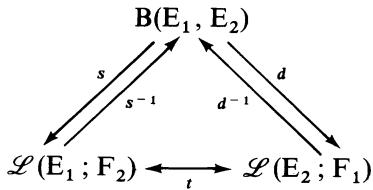
\includegraphics[keepaspectratio]{images/part001_08254dbd.jpg}}

where t is the isomorphism of transposition (II, p.~46, prop. 5 and corollary). In view of the definition of weak topologies on \(F_{1}\) and \(F_{2}\) , it is immediate that when \(\mathbf{B}(\mathbf{E}_{1}, \mathbf{E}_{2})\) , \(\mathcal{L}(\mathbf{E}_{1}; \mathbf{E}_{2})\) and \(\mathcal{L}(\mathbf{E}_{2}; \mathbf{F}_{1})\) are assigned the topology of simple convergence, the isomorphisms of diagram (3) are topological vector space isomorphisms.

\subsection{Separately continuous bilinear mappings on a product of Fréchet spaces}

PROPOSITION 2. --- Let E, F and G be three locally convex spaces. Suppose that E and F are metrizable and E is barrelled. Let H be a set of separately continuous bilinear mappings from E × F into G. Suppose that for every x ∈ E, the set of mappings u(x, .) from F into G, where u runs through H, is equicontinuous. Then H is equicontinuous.

Let \(\mathrm{U}_n(\text{resp. } \mathrm{V}_n)\) be a fundamental sequence of neighbourhoods of 0 in E (resp. F). If H is not equicontinuous, there exists a closed, convex, balanced neighbourhood W of 0 in G such that for all \(n\) , \(\mathrm{H}(\mathrm{U}_n \times \mathrm{V}_n)\) is not contained in W. There exists then a sequence of pairs \((x_n, y_n) \in \mathrm{U}_n \times \mathrm{V}_n\) , and a sequence \((u_n)\) of elements of H, such that \(u_n(x_n, y_n) \notin \mathrm{W}\) . Let \(p\) be the gauge of W. For every \(y \in \mathrm{F}\) and every \(u \in \mathrm{H}\) , the mapping \(u(., y)\) from E into G is continuous, hence \(p \circ u(., y)\) is a continuous seminorm on E. On the other hand, for every \(x \in \mathrm{E}\) , the set of mappings \(u(x, .)\) for \(u \in \mathrm{H}\) is equicontinuous; since the sequence \((y_n)\) tends to 0, it is bounded, and the set of all \(u(x, y_n)\) , for \(n \geqslant 0\) and \(u \in \mathrm{H}\) , is bounded (III, p.~22, prop. 9). It follows from this that the function \(p'(x) = \sup_{\substack{u \in \mathrm{H} \\ n \geqslant 0}} p(u(x, y_n))\) is a lower semi-continuous semi-

norm (finite) on E. Since E is barrelled, \(p'\) is continuous (III, p.~24, corollary). Since \((x_{n})\) tends to 0 in E, \(p'(x_{n})\) tends to 0, so that we have \(p'(x_{n}) \leqslant 1\) if n is large enough; but then \(p(u_{n}(x_{n}, y_{n})) \leqslant p'(x_{n}) \leqslant 1\) , hence \(u_{n}(x_{n}, y_{n}) \in \mathbf{W}\) , which contradicts the hypothesis on \(u_{n}, x_{n}, y_{n}\) .

COROLLARY 1. --- Let E and F be two Fréchet spaces, and G a locally convex space. Every separately continuous bilinear mapping from E × F into G is continuous.

In fact, every Fréchet space is barrelled (III, p.~25, corollary).

Let E and F be two locally convex spaces. We use \(\mathcal{B}(\mathrm{E},\mathrm{F})\) to denote the space of continuous bilinear forms on \(E \times F\) , with the topology of uniform convergence on sets of the form \(A \times B\) , where A (resp. B) is bounded in E (resp. F). The formula

\[
u (x, y) = \langle y, \phi (u) (x) \rangle
\]

(for \(x \in \mathrm{E}\) , \(y \in \mathrm{F}\) and \(u \in \mathcal{B}(\mathrm{E}, \mathrm{F})\) ) defines a continuous linear injective mapping \(\phi\) from \(\mathcal{B}(\mathrm{E}, \mathrm{F})\) into \(\mathcal{L}_b(\mathrm{E}; \mathrm{F}_b')\) .

COROLLARY 2. --- Suppose that E and F are metrizable and that E is barrelled. Then \(\phi\) is a topological vector space isomorphism from \(\mathcal{B}(\mathrm{E},\mathrm{F})\) onto \(\mathcal{L}_b(\mathrm{E};\mathrm{F}_b')\) .

Let \(f \in \mathcal{L}_b(\mathrm{E}; \mathrm{F}_b')\) . Put \(u(x, y) = \langle y, f(x) \rangle\) for \(x \in \mathrm{E}\) and \(y \in \mathrm{F}\) . The bilinear form \(u\) on \(\mathrm{E} \times \mathrm{F}\) is separately continuous; by prop. 2, it belongs to \(\mathcal{B}(\mathrm{E}, \mathrm{F})\) , and we have \(f = \phi(u)\) . Hence \(\phi\) is a linear bijection from \(\mathcal{B}(\mathrm{E}, \mathrm{F})\) onto \(\mathcal{L}_b(\mathrm{E}; \mathrm{F}_b')\) . It is immediate that \(\phi\) is bicontinuous, hence cor. 2 follows.

\subsection{Hypocontinuous bilinear mappings}

In what follows, we shall define a notion which is intermediate between that of a continuous bilinear mapping and that of a separately continuous bilinear mapping.

PROPOSITION 3. --- Let E, F, G be three locally convex spaces, S a family of bounded subsets of E. Let u be a separately continuous bilinear mapping from E × F into G. The following properties are equivalent :

\begin{enumerate}
\def\labelenumi{\alph{enumi})}
\item
  For every neighbourhood \(\mathbf{W}\) of 0 in \(\mathbf{G}\) and every set \(\mathbf{M} \in \mathfrak{S}\) , there exists a neighbourhood \(\mathbf{V}\) of 0 in \(\mathbf{F}\) such that \(u(\mathbf{M} \times \mathbf{V}) \subset \mathbf{W}\) .
\item
  For every set \(\mathbf{M} \in \mathfrak{S}\) , the image of \(\mathbf{M}\) under the mapping \(x \mapsto u(x, .)\) is an equicontinuous subset of \(\mathcal{L}(\mathrm{F}; \mathrm{G})\) .
\item
  The mapping \(y \mapsto u(., y)\) from \(\mathbf{F}\) into \(\mathcal{L}_{\mathfrak{S}}(\mathbf{E}; \mathbf{G})\) is continuous.
\item
  expresses that \(y \mapsto u(., y)\) is continuous at the point 0, on account of the definition of neighbourhoods of 0 in \(\mathcal{L}_{\mathfrak{S}}(\mathrm{E}; \mathrm{G})\) (III, p.~13); likewise a) expresses that the image of M under the mapping \(x \mapsto u(x, .)\) is equicontinuous at the point 0 (III, p.~16).
\end{enumerate}

DEFINITION 2. --- Let u be a bilinear mapping from E × F into G. We say that u is S-hypocontinuous if u is separately continuous and if it verifies one of the equivalent conditions a), b), c) of prop. 3.

The condition \(c)\) of prop. 3 shows that the notion of \(\mathfrak{S}\) -hypocontinuous bilinear mapping depends on \(\mathfrak{S}\) only through the \(\mathfrak{S}\) -topology on \(\mathcal{L}(\mathrm{E},\mathrm{G})\) .

For every set T of bounded subsets of F, we define similarly the notion of T-hypo-continuous mapping, by interchanging the roles of E and F in prop. 3. A separately continuous bilinear mapping u is said to be \((\mathfrak{S}, \mathfrak{T})\) -hypocontinuous if it is both S-hypocontinuous and T-hypocontinuous.

Every continuous bilinear mapping from \(E \times F\) into G is \((\mathfrak{S}, \mathfrak{T})\) -hypocontinuous for every pair \((\mathfrak{S}, \mathfrak{T})\) of sets of bounded subsets: for every neighbourhood W of 0 in G, there exists a neighbourhood U of 0 in E and a neighbourhood V of 0 in F such that \(u(U \times V) \subset W\) ; since every set \(M \in S\) is bounded, there exists \(\lambda > 0\) such that \(\lambda M \subset V\) , and so

\[
u (\mathbf {M} \times \lambda \mathbf {V}) = u (\lambda \mathbf {M} \times \mathbf {V}) \subset u (\mathbf {U} \times \mathbf {V}) \subset \mathbf {W}.
\]

The converse is in general false (III, p.~47, exerc. 3).

PROPOSITION 4. --- Let u be a S-hypocontinuous bilinear mapping from E × F into G. For every set M ∈ S, the restriction of u to M × F is continuous, and u(M × Q) is bounded in G for every bounded subset Q of F.

The first assertion follows from cor. 3 of GT, X, § 2, No.~1. Let W be a neighbourhood of 0 in G; there exists, by hypothesis, a neighbourhood V of 0 in F such that \(u(\mathbf{M} \times \mathbf{V}) \subset \mathbf{W}\) . Since there exists \(\lambda \neq 0\) such that \(\lambda \mathbf{Q} \subset \mathbf{V}\) , we have \(\lambda u(\mathbf{M} \times \mathbf{Q}) = u(\mathbf{M} \times \lambda \mathbf{Q}) \subset \mathbf{W}\) , and this proves the second part of the proposition.

PROPOSITION 5. --- Let u be a (S, T)-hypocontinuous bilinear mapping from E × F into G. For every pair of sets M ∈ S, N ∈ T, u is uniformly continuous on M × N. The proposition follows immediately from prop. 2 of GT, X, § 2, No.~1 and prop. 5 of GT, X, § 2, No.~2.

PROPOSITION 6. --- If F is a barrelled space, every separately continuous bilinear mapping u from E × F into a locally convex space G is S-hypocontinuous for every set S of bounded subsets of E.

In other words, the linear mapping \(y \mapsto u(., y)\) from \(F\) into \(\mathcal{L}_b(E; G)\) is continuous. It is enough (III, p.~30, prop. 3) to prove that the image of every bounded subset \(M\) of \(E\) under \(x \mapsto u(x, .)\) is equicontinuous in \(\mathcal{L}(F; G)\) . But, by virtue of prop. 1 (III, p.~28) this image is a simply bounded subset of \(\mathcal{L}(F; G)\) , and since \(F\) is barrelled, every simply bounded subset of \(\mathcal{L}(F; G)\) is equicontinuous (III, p.~25, th. 1).

Remark. --- Suppose the topology of F is the finest locally convex topology on F for which the linear mappings \(h_{\alpha}:F_{\alpha}\to F\) are continuous (II, p.~27). Then condition c) of prop. 3 (III, p.~30) shows that if E and G are locally convex, then the bilinear mapping \(u:E\times F\to G\) is S-hypocontinuous if and only if each of the bilinear mappings

\[
(x, y _ {\alpha}) \mapsto u (x, h _ {\alpha} (y _ {\alpha}))
\]

from \(\mathbf{E} \times \mathbf{F}_{\alpha}\) into \(\mathbf{G}\) is \(\mathfrak{S}\) -hypocontinuous.

Now suppose that \(\mathbf{E}\) is a locally convex space which is the strict inductive limit of an increasing sequence \((\mathbf{E}_n)\) of closed vector subspaces of \(\mathbf{E}\) (II, p.~33); then every set \(\mathbf{M} \in \mathfrak{S}\) is contained in one of the \(\mathbf{E}_n\) and is bounded in this subspace (III, p.~5, prop. 6). We denote by \(\mathfrak{S}_n\) the family of all subsets belonging to \(\mathfrak{S}\) contained in \(\mathbf{E}_n\) .

Condition a) of prop. 3 (III, p.~30) shows that for a bilinear mapping \(u: \mathrm{E} \times \mathrm{F} \to \mathrm{G}\) to be \(\mathfrak{S}\) -hypocontinuous, it is necessary and sufficient that each of the restrictions \(u_n: \mathrm{E}_n \times \mathrm{F} \to \mathrm{G}\) of \(u\) is \(\mathfrak{S}_n\) -hypocontinuous.

\subsection{Extension of a hypocontinuous bilinear mapping}

PROPOSITION 7. --- Let E, F, G be three locally convex spaces, G being assumed Hausdorff; let \(E_{0}\) (resp. \(F_{0}\) ) be a dense vector subspace of E (resp. F). Let u be a separately continuous bilinear mapping from \(E \times F\) into G.

\begin{enumerate}
\def\labelenumi{\arabic{enumi})}
\item
  If \(u(\mathrm{E}_0 \times \mathrm{F}_0) = \{0\}\) , then \(u = 0\) .
\item
  Let \(\mathfrak{S}_0\) be a family of bounded subsets of \(\mathbf{E}_0\) ; if the restriction of \(u\) to \(\mathbf{E}_0 \times \mathbf{F}_0\) is \(\mathfrak{S}_0\) -hypocontinuous then so is \(u\) .
\item
  By hypothesis, for all \(x \in \mathrm{E}_0\) , the continuous linear mapping \(u(x, .)\) is null on \(\mathrm{F}_0\) , hence on \(\mathrm{F}\) : therefore for all \(y \in \mathrm{F}\) , the continuous linear mapping \(u(., y)\) is null on \(\mathrm{E}_0\) , hence on \(\mathrm{E}\) . This proves that \(u = 0\) .
\item
  For every closed neighbourhood W of 0 in G and for every set \(\mathbf{M} \in \mathfrak{S}_0\) , there exists, by hypothesis, a neighbourhood V of 0 in \(\mathrm{F}_0\) such that \(u(\mathbf{M} \times \mathbf{V}) \subset \mathbf{W}\) . But \(\overline{\mathbf{V}}\) is a neighbourhood of 0 in F; for every \(x \in \mathbf{M}\) , the relation \(u(\{x\} \times \mathbf{V}) \subset \mathbf{W}\) implies that \(u(\{x\} \times \overline{\mathbf{V}}) \subset \mathbf{W}\) , since \(u(x, .)\) is continuous and W is closed; therefore \(u(\mathbf{M} \times \overline{\mathbf{V}}) \subset \mathbf{W}\) , which proves that \(u\) is \(\mathfrak{S}_0\) -hypocontinuous.
\end{enumerate}

PROPOSITION 8. --- Let E, F, G be three locally convex spaces; assume that G is Hausdorff and quasi-complete. Let \(E_{0}\) (resp. \(F_{0}\) ) be a dense vector subspace of E (resp. F), \(S_{0}\) (resp. \(T_{0}\) ) a family of bounded subsets of \(E_{0}\) (resp. \(F_{0}\) ) such that every point of E (resp. F) is in the closure of an element of \(S_{0}\) (resp. \(T_{0}\) ). Then every \((\mathfrak{S}_{0}, \mathfrak{T}_{0})\) -hypocontinuous bilinear mapping u from \(E_{0} \times F_{0}\) into G extends uniquely to a separately continuous bilinear mapping \(\overline{u}\) from E × F into G and \(\overline{u}\) is \((\mathfrak{S}_{0}, \mathfrak{T}_{0})\) -hypocontinuous.

The uniqueness and hypocontinuity of \(\overline{u}\) follows from prop. 7; it remains to prove the existence of \(\overline{u}\) . For every \(y' \in F_{0}\) , the continuous linear mapping \(x' \mapsto u(x', y')\) from \(E_{0}\) into G extends uniquely to a continuous linear mapping \(x \mapsto u_{1}(x, y')\) from E into G (III, p.~8, prop. 10). It follows immediately that for every \(x \in E\) , the mapping \(y' \mapsto u_{1}(x, y')\) from \(F_{0}\) into G is linear; and we shall show that it is continuous. By hypothesis, there exists \(M \in S_{0}\) , such that \(x \in M\) . For every closed neighbourhood W of 0 in G, there exists, by hypothesis, a neighbourhood V of 0 in \(F_{0}\) such that \(u(M \times V) \subset W\) ; since \(x \mapsto u_{1}(x, y')\) is continuous, we deduce that \(u_{1}(\overline{\mathbf{M}} \times \mathbf{V}) \subset \mathbf{W}\) , and in particular \(u_{1}(x, y') \in \mathbf{W}\) for all \(y' \in V\) . This establishes our assertion. By virtue of prop. 7, the bilinear map \(u_{1}\) from \(E \times F_{0}\) into G is \((\mathfrak{S}_{0}, \mathfrak{T}_{0})\) -hypocontinuous. We end the proof by interchanging the roles of E and F in the first part of the proof, applied to \(u_{1}\) .
